% =====================================================================
%  LipScribe: Technical Implementation and System Development Document
%  Computer Vision and Deep Learning -- Group 4
%  Uganda Christian University
%
%  Compiles with pdfLaTeX, XeLaTeX, LuaLaTeX or Tectonic (see README.md).
% =====================================================================
\documentclass[11pt,a4paper]{article}

% ---------------------------------------------------------------- engine
\usepackage{iftex}
\ifPDFTeX
  \usepackage[T1]{fontenc}
  \usepackage[utf8]{inputenc}
\fi
\usepackage{lmodern}
\usepackage{microtype}
\setlength{\emergencystretch}{3em}

% ---------------------------------------------------------------- layout
\usepackage[a4paper,margin=2.5cm,headheight=14pt]{geometry}
\usepackage{setspace}
\setstretch{1.12}
\usepackage[parfill]{parskip}
\usepackage{titlesec}
\usepackage{fancyhdr}
\usepackage{enumitem}
\setlist{itemsep=2pt,topsep=4pt}

% ---------------------------------------------------------------- maths
\usepackage{amsmath,amssymb,bm}

% ---------------------------------------------------------------- tables, figures
\usepackage{graphicx}
\usepackage{booktabs}
\usepackage{tabularx}
\renewcommand{\tabularxcolumn}[1]{>{\raggedright\arraybackslash}p{#1}}
\usepackage{array}
\usepackage{longtable}
\usepackage{multirow}
\usepackage{float}
\usepackage[font=small,labelfont={bf,sf},skip=6pt]{caption}
\usepackage{xcolor}
\usepackage{tikz}
\usetikzlibrary{positioning,arrows.meta,fit,backgrounds,calc,shapes.geometric}

% ---------------------------------------------------------------- code & algorithms
\usepackage{listings}
\usepackage{algorithm}
\usepackage{algpseudocode}

% ---------------------------------------------------------------- colours
\definecolor{lsblue}{RGB}{31,73,125}
\definecolor{lsgrey}{RGB}{110,110,110}
\definecolor{lsaudio}{RGB}{214,234,248}
\definecolor{lsvisual}{RGB}{252,228,214}
\definecolor{lsfuse}{RGB}{226,239,218}
\definecolor{lsout}{RGB}{237,231,246}
\definecolor{codebg}{RGB}{247,247,247}

% ---------------------------------------------------------------- headings
\titleformat{\section}{\Large\sffamily\bfseries\color{lsblue}}{\thesection}{0.8em}{}
\titleformat{\subsection}{\large\sffamily\bfseries\color{lsblue}}{\thesubsection}{0.8em}{}
\titleformat{\subsubsection}{\normalsize\sffamily\bfseries}{\thesubsubsection}{0.8em}{}
\titlespacing*{\section}{0pt}{18pt}{8pt}
\titlespacing*{\subsection}{0pt}{12pt}{5pt}
\titlespacing*{\subsubsection}{0pt}{9pt}{3pt}

% ---------------------------------------------------------------- headers / footers
\pagestyle{fancy}
\fancyhf{}
\fancyhead[L]{\small\sffamily\color{lsgrey}LipScribe -- Technical Implementation Document}
\fancyhead[R]{\small\sffamily\color{lsgrey}CVDL Group 4}
\fancyfoot[C]{\small\sffamily\thepage}
\renewcommand{\headrulewidth}{0.4pt}
\fancypagestyle{plain}{\fancyhf{}\fancyfoot[C]{\small\sffamily\thepage}\renewcommand{\headrulewidth}{0pt}}

% ---------------------------------------------------------------- listings style
\lstdefinestyle{lipscribe}{
  basicstyle=\ttfamily\footnotesize,
  backgroundcolor=\color{codebg},
  keywordstyle=\color{lsblue}\bfseries,
  commentstyle=\color{lsgrey}\itshape,
  stringstyle=\color{red!50!black},
  frame=single, rulecolor=\color{black!15},
  breaklines=true, columns=fullflexible,
  showstringspaces=false, tabsize=2,
  xleftmargin=4pt, xrightmargin=4pt
}
\lstset{style=lipscribe}

% ---------------------------------------------------------------- custom boxes
% Labels used throughout to separate the source of each statement.
\newcommand{\spec}{\textsf{\textbf{\color{lsblue}[Proposal]}}}
\newcommand{\rec}{\textsf{\textbf{\color{green!40!black}[Recommended]}}}
\newcommand{\tbd}{\textsf{\textbf{\color{red!60!black}[To be decided]}}}
\newcommand{\shape}[1]{$\langle #1 \rangle$}

% ---------------------------------------------------------------- hyperlinks (load last)
\usepackage[hidelinks]{hyperref}
\hypersetup{
  pdftitle={LipScribe: Technical Implementation and System Development Document},
  pdfauthor={Migisha, Opol, Ainomugisha, Namugenyi, Naamaye, Isabelle},
  pdfsubject={Audio-visual speech recognition implementation plan},
  hypertexnames=false
}
\usepackage[nameinlink,capitalise]{cleveref}

\renewcommand{\algorithmicrequire}{\textbf{Input:}}
\renewcommand{\algorithmicensure}{\textbf{Output:}}

% =====================================================================
\begin{document}

% ---------------------------------------------------------------- title page
\begin{titlepage}
\thispagestyle{empty}
\centering
\vspace*{1.2cm}

{\sffamily\large\color{lsgrey} Computer Vision and Deep Learning \quad$\cdot$\quad Group 4\par}
\vspace{1.6cm}

{\sffamily\bfseries\fontsize{30}{36}\selectfont\color{lsblue} LipScribe\par}
\vspace{0.4cm}
{\sffamily\Large Technical Implementation and\\[2pt] System Development Document\par}
\vspace{0.6cm}
{\itshape\large Lip-Assisted Speech Recognition for Robust Live Captioning\par}

\vspace{1.4cm}
{\color{lsblue}\rule{0.6\textwidth}{0.8pt}}
\vspace{1.0cm}

{\sffamily\bfseries Team members\par}
\vspace{0.3cm}
\begin{tabular}{ll}
Cole Rodney Migisha        & \texttt{b29657} \\
Charis Opol                & \texttt{b29654} \\
Ainomugisha Faith          & \texttt{b27518} \\
Lisa Lusinga Namugenyi     & \texttt{b30300} \\
Ansasire Nehum Naamaye     & \texttt{b29785} \\
Wakisa Isabelle            & \texttt{b30311} \\
\end{tabular}

\vspace{1.0cm}
{\small Student e-mail: \texttt{<id>@students.ucu.ac.ug}\par}

\vfill
{\sffamily Department of Computer Science\\
Uganda Christian University, Mukono, Uganda\par}
\vspace{0.5cm}
{\sffamily October 2026\par}
\vspace{0.6cm}

\begin{minipage}{0.86\textwidth}
\small\color{lsgrey}
\textbf{Status of this document.} This document describes how the system
proposed in the LipScribe project proposal will be implemented. It reports
planned work, not completed work: no experimental results are presented, and
all numerical settings that the proposal does not fix are marked as
recommendations to be confirmed during development.
\end{minipage}
\end{titlepage}


\pagenumbering{roman}
\tableofcontents
\clearpage
\listoffigures
\listoftables
\listofalgorithms
\clearpage
% ---------------------------------------------------------------- abbreviations
\section*{List of Abbreviations}
\addcontentsline{toc}{section}{List of Abbreviations}

\begin{longtable}{@{}p{0.18\textwidth}p{0.76\textwidth}@{}}
\toprule
\textbf{Abbreviation} & \textbf{Meaning} \\
\midrule
\endhead
AMP      & Automatic Mixed Precision \\
ASR      & Automatic Speech Recognition \\
AVSR     & Audio-Visual Speech Recognition \\
BiLSTM   & Bidirectional Long Short-Term Memory network \\
BN       & Batch Normalisation \\
CER      & Character Error Rate \\
CNN      & Convolutional Neural Network \\
CTC      & Connectionist Temporal Classification \\
DCT      & Discrete Cosine Transform \\
FPS      & Frames Per Second \\
GPU      & Graphics Processing Unit \\
LM       & Language Model \\
LSTM     & Long Short-Term Memory \\
MFCC     & Mel-Frequency Cepstral Coefficients \\
MHA      & Multi-Head Attention \\
MUSAN    & Music, Speech and Noise corpus \\
RMS      & Root Mean Square \\
RQ       & Research Question \\
RTF      & Real-Time Factor \\
SNR      & Signal-to-Noise Ratio \\
STFT     & Short-Time Fourier Transform \\
UI       & User Interface \\
WER      & Word Error Rate \\
\bottomrule
\end{longtable}

\subsection*{Statement labels used in this document}
To separate fixed project requirements from engineering choices, statements
are tagged as follows:

\begin{description}[leftmargin=3.2cm,style=nextline]
  \item[\spec] Specified by the LipScribe project proposal. These items define
        the intended system and are not changed without team agreement.
  \item[\rec] An implementation decision recommended in this document. It is
        a practical starting point and may be revised on evidence.
  \item[\tbd] An open question that will be settled experimentally or by the
        team during development.
\end{description}

\clearpage

\pagenumbering{arabic}
% =====================================================================
\section{Introduction and Implementation Overview}
\label{sec:intro}
% =====================================================================

\subsection{Purpose of LipScribe}
LipScribe is an audio-visual speech recognition (AVSR) system that produces
text captions from a speaker's voice and lip movements together. Conventional
automatic speech recognition (ASR) performs well in quiet rooms but degrades
sharply when background noise, overlapping speakers or muffled speech corrupt
the audio signal. Lip movements are unaffected by acoustic noise, so a model
that also watches the mouth retains a usable source of evidence when the audio
becomes unreliable~\cite{li2023,afouras2022}. The implementation described here
therefore aims to build a recogniser whose accuracy degrades more gracefully in
noise than an audio-only system.

The proposal identifies deaf and hard-of-hearing people as the primary
beneficiaries, with lectures, meetings and public spaces as the intended
settings \spec. These users depend on captions being correct rather than merely
fast, so the implementation prioritises measurable transcription quality across
noise levels and treats latency as a constraint to be measured, not assumed.

\subsection{Problem statement and objectives}
The proposal states the central problem as: \emph{how can transcription be
improved by combining audio understanding with lip reading so that captions
remain usable even when the audio channel is severely degraded?} \spec. It
defines four objectives, each linked to a research question (RQ). \Cref{tab:objectives}
maps each objective to the part of the implementation that addresses it and
states whether that part belongs to the core system.

\begin{table}[H]
\centering
\caption{Mapping of proposal objectives to implementation components.}
\label{tab:objectives}
\small
\begin{tabularx}{\textwidth}{@{}p{3.4cm}X p{1.9cm}@{}}
\toprule
\textbf{Objective (RQ)} & \textbf{Implementation component} & \textbf{Scope} \\
\midrule
1. Disambiguate homophenes (RQ1) &
Cross-modal attention lets acoustic context resolve visually identical lip
shapes; temporal modelling over neighbouring frames (\cref{sec:model}). &
Core \\
2. Model temporal word sequences (RQ2) &
3D-CNN front-end, BiLSTM encoders and CTC training map frame sequences to
whole sentences (\cref{sec:visual,sec:audio,sec:model}). &
Core \\
3. Detect emotion from speaking style (RQ3) &
Separate landmark-based classifier trained on an emotion-labelled dataset
(\cref{sec:extensions}). &
Extension \\
4. Identify the spoken language (RQ4) &
Separate language-identification head trained on multilingual data
(\cref{sec:extensions}). &
Extension \\
\bottomrule
\end{tabularx}
\end{table}

\subsection{End-to-end workflow}
At run time the system executes the same sequence of stages for every segment
of input. \Cref{fig:workflow} summarises them; \cref{sec:architecture}
describes each stage as a software module.

\begin{enumerate}
  \item \textbf{Capture} synchronised video frames and audio samples from a
        camera and microphone, or read them from a recorded clip.
  \item \textbf{Detect the face} in every frame with MediaPipe Face
        Mesh~\cite{kartynnik2019,lugaresi2019} and locate the lip landmarks.
  \item \textbf{Extract the mouth sequence} by cropping a fixed-size region
        around the lips in each frame.
  \item \textbf{Extract audio features} (log-Mel spectrograms, optionally MFCCs)
        from the waveform.
  \item \textbf{Encode each modality} with its own neural encoder: a 3D-CNN and
        BiLSTM for video, and a BiLSTM for audio.
  \item \textbf{Fuse} the two encoded sequences with cross-modal attention.
  \item \textbf{Decode} the fused sequence into characters with a CTC output
        layer and beam search.
  \item \textbf{Display} the resulting text as a caption.
\end{enumerate}

\begin{figure}[H]
\centering
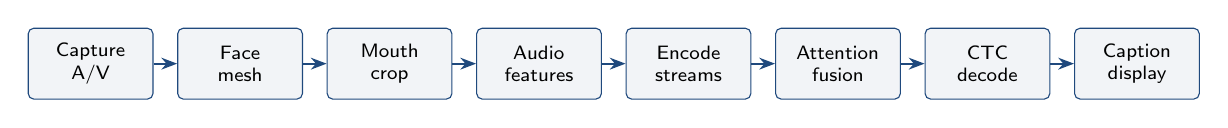
\begin{tikzpicture}[
  node distance=3mm,
  st/.style={draw=lsblue, rounded corners=2pt, fill=lsblue!6, align=center,
             font=\scriptsize\sffamily, minimum height=9mm, text width=13.5mm},
  ar/.style={-{Stealth[length=2mm]}, thick, lsblue}]
\node[st] (a) {Capture\\A/V};
\node[st, right=of a] (b) {Face\\mesh};
\node[st, right=of b] (c) {Mouth\\crop};
\node[st, right=of c] (d) {Audio\\features};
\node[st, right=of d] (e) {Encode\\streams};
\node[st, right=of e] (f) {Attention\\fusion};
\node[st, right=of f] (g) {CTC\\decode};
\node[st, right=of g] (h) {Caption\\display};
\foreach \x/\y in {a/b,b/c,c/d,d/e,e/f,f/g,g/h} \draw[ar] (\x) -- (\y);
\end{tikzpicture}
\caption{The eight stages of the LipScribe processing workflow.}
\label{fig:workflow}
\end{figure}

\subsection{Scope of the initial implementation}
The core deliverable is the audio-visual speech recogniser and a captioning
demonstration built on it. It covers objectives~1 and~2 and the evaluation
plan in the proposal: training on the GRID corpus~\cite{cooke2006} with
MUSAN noise~\cite{snyder2015} added at clean, 10, 5, 0 and $-5$\,dB SNR, and
reporting WER and CER on held-out speakers \spec.

Emotion detection and language identification (objectives~3 and~4) are not
part of the core architecture in this plan. GRID provides no emotion labels
and contains a single language, so neither task can be trained or evaluated
on it alone. \Cref{sec:extensions} describes how each could be investigated as
a separate module with its own data and evaluation, to be attempted only after
the core system works (\cref{sec:schedule}). Keeping them separate prevents
unvalidated extensions from delaying or obscuring the main result.

\subsection{Structure of this document}
\Cref{sec:architecture,sec:stack} define the system architecture and
technology stack. \Cref{sec:dataset,sec:visual,sec:audio} describe the data
and the two preprocessing pipelines. \Cref{sec:model,sec:training,sec:evaluation}
specify the model, its training and its evaluation. \Cref{sec:application}
covers the live captioning application, \cref{sec:extensions} the optional
extensions, and \cref{sec:schedule,sec:risks,sec:deliverables} the schedule,
risks and deliverables.

% =====================================================================
\section{System Architecture and Design}
\label{sec:architecture}
% =====================================================================

\subsection{Architectural overview}
LipScribe is organised as a pipeline of independent modules connected by
well-defined tensor interfaces. Two parallel streams process the visual and
audio inputs; a fusion module combines their encoded sequences; and a
CTC-based head turns the fused sequence into text. \Cref{fig:architecture}
shows the complete architecture. Each module can be developed, tested and
replaced on its own, which lets team members work in parallel and lets the
baselines in \cref{sec:training} reuse the same components.

\begin{figure}[p]
\centering
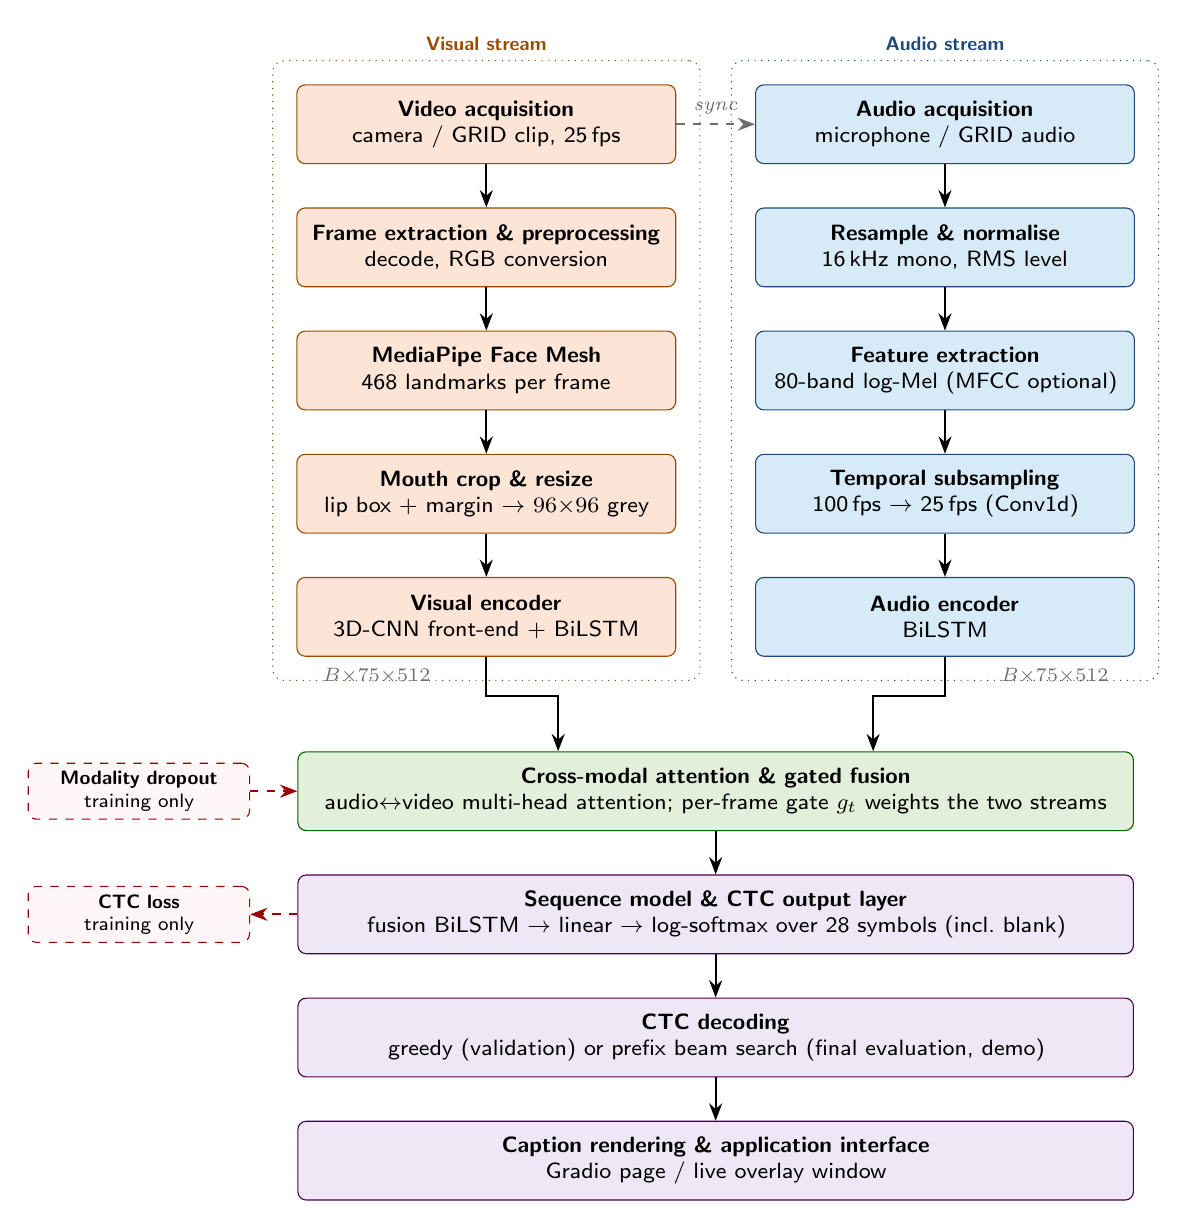
\begin{tikzpicture}[
  node distance=5.5mm and 10mm,
  box/.style={draw, rounded corners=3pt, align=center, font=\footnotesize\sffamily,
              minimum height=10mm, text width=46mm, inner sep=3pt},
  vis/.style={box, fill=lsvisual, draw=orange!60!black},
  aud/.style={box, fill=lsaudio, draw=lsblue},
  fus/.style={box, fill=lsfuse, draw=green!40!black, text width=104mm},
  outp/.style={box, fill=lsout, draw=violet!60!black, text width=104mm},
  train/.style={draw=red!60!black, dashed, rounded corners=3pt, align=center,
                font=\scriptsize\sffamily, fill=red!3, text width=26mm, inner sep=3pt},
  ar/.style={-{Stealth[length=2.2mm]}, thick},
  lab/.style={font=\scriptsize\itshape, text=lsgrey}]

% ---- visual column
\node[vis] (v0) {\textbf{Video acquisition}\\camera / GRID clip, 25\,fps};
\node[vis, below=of v0] (v1) {\textbf{Frame extraction \& preprocessing}\\decode, RGB conversion};
\node[vis, below=of v1] (v2) {\textbf{MediaPipe Face Mesh}\\468 landmarks per frame};
\node[vis, below=of v2] (v3) {\textbf{Mouth crop \& resize}\\lip box + margin $\rightarrow$ $96{\times}96$ grey};
\node[vis, below=of v3] (v4) {\textbf{Visual encoder}\\3D-CNN front-end + BiLSTM};

% ---- audio column
\node[aud, right=of v0] (a0) {\textbf{Audio acquisition}\\microphone / GRID audio};
\node[aud, below=of a0] (a1) {\textbf{Resample \& normalise}\\16\,kHz mono, RMS level};
\node[aud, below=of a1] (a2) {\textbf{Feature extraction}\\80-band log-Mel (MFCC optional)};
\node[aud, below=of a2] (a3) {\textbf{Temporal subsampling}\\100\,fps $\rightarrow$ 25\,fps (Conv1d)};
\node[aud, below=of a3] (a4) {\textbf{Audio encoder}\\BiLSTM};

% ---- fusion and output
\node[fus, below=12mm of $(v4.south)!0.5!(a4.south)$] (f)
  {\textbf{Cross-modal attention \& gated fusion}\\
   audio$\leftrightarrow$video multi-head attention; per-frame gate $g_t$ weights the two streams};
\node[outp, below=of f] (c) {\textbf{Sequence model \& CTC output layer}\\fusion BiLSTM $\rightarrow$ linear $\rightarrow$ log-softmax over 28 symbols (incl.\ blank)};
\node[outp, below=of c] (d) {\textbf{CTC decoding}\\greedy (validation) or prefix beam search (final evaluation, demo)};
\node[outp, below=of d] (o) {\textbf{Caption rendering \& application interface}\\Gradio page / live overlay window};

% ---- arrows
\foreach \x/\y in {v0/v1,v1/v2,v2/v3,v3/v4,a0/a1,a1/a2,a2/a3,a3/a4,f/c,c/d,d/o}
  \draw[ar] (\x) -- (\y);
\draw[ar] (v4.south) -- ++(0,-5mm) -| ([xshift=-20mm]f.north);
\draw[ar] (a4.south) -- ++(0,-5mm) -| ([xshift=20mm]f.north);
\draw[ar, dashed, lsgrey] (v0.east) -- node[above, lab]{sync} (a0.west);

% ---- training-only components
\node[train, left=6mm of f] (md) {\textbf{Modality dropout}\\training only};
\draw[ar, red!60!black, dashed] (md) -- (f);
\node[train, left=6mm of c] (loss) {\textbf{CTC loss}\\training only};
\draw[ar, red!60!black, dashed] (c) -- (loss);

% ---- tensor annotations
\node[lab, right=1mm of v4.south east, anchor=north west] {};
\node[lab, anchor=west] at ($(v4.south)+(-22mm,-2.5mm)$) {$B{\times}75{\times}512$};
\node[lab, anchor=east] at ($(a4.south)+(22mm,-2.5mm)$) {$B{\times}75{\times}512$};

% ---- stream labels
\begin{scope}[on background layer]
  \node[draw=orange!60!black, dotted, rounded corners, fit=(v0)(v4), inner sep=3mm,
        label={[font=\scriptsize\sffamily\bfseries, text=orange!60!black]above:Visual stream}] {};
  \node[draw=lsblue, dotted, rounded corners, fit=(a0)(a4), inner sep=3mm,
        label={[font=\scriptsize\sffamily\bfseries, text=lsblue]above:Audio stream}] {};
\end{scope}
\end{tikzpicture}
\caption[LipScribe system architecture]{LipScribe system architecture. The
visual (left) and audio (right) streams are processed independently, fused by
cross-modal attention and decoded with CTC. Dashed red components are active
only during training. Tensor sizes assume a 3\,s GRID clip ($T=75$ video
frames) and the recommended configuration of \cref{sec:model}.}
\label{fig:architecture}
\end{figure}

\subsection{Module descriptions}
\Cref{tab:modules} lists every module with its inputs, outputs and
connections. Interfaces are expressed as tensor shapes so that each module can
be tested in isolation; $B$ is the batch size, $T$ the number of video frames,
and $T_a$ the number of audio feature frames.

{\small
\setlength{\tabcolsep}{4pt}
\begin{longtable}{@{}p{2.4cm}p{3.4cm}p{2.9cm}p{2.9cm}p{2.7cm}@{}}
\caption{Module responsibilities and interfaces.}\label{tab:modules}\\
\toprule
\textbf{Module} & \textbf{Purpose} & \textbf{Input} & \textbf{Output} & \textbf{Connects to} \\
\midrule
\endfirsthead
\multicolumn{5}{@{}l}{\small\itshape \Cref{tab:modules} continued}\\
\toprule
\textbf{Module} & \textbf{Purpose} & \textbf{Input} & \textbf{Output} & \textbf{Connects to} \\
\midrule
\endhead
\bottomrule
\endfoot
A/V acquisition & Read synchronised frames and samples from a file or device &
Video file / camera, audio file / microphone & Frame list with timestamps; waveform &
Frame extraction, resampling \\
Frame extraction & Decode frames, convert colour space, enforce frame rate &
Raw frames & RGB frames \shape{T,H,W,3} & Face Mesh \\
MediaPipe Face Mesh & Locate 468 facial landmarks per frame~\cite{kartynnik2019} &
RGB frame & Landmark array \shape{468,3} or ``not found'' & Mouth crop \\
Mouth crop \& resize & Extract a stable, fixed-size lip region &
Frame and lip landmarks & Grey crop \shape{96,96}, validity flag & Visual encoder \\
Visual encoder & Model lip appearance and motion over time &
Clip \shape{B,1,T,96,96} & Sequence \shape{B,T,512} & Fusion \\
Audio resample \& normalise & Standardise sample rate, channels and level &
Waveform at source rate & 16\,kHz mono waveform & Feature extraction \\
Feature extraction & Compute time--frequency representation &
Waveform \shape{N} & Log-Mel \shape{T_a,80}, $T_a\approx 4T$ & Audio encoder \\
Audio encoder & Subsample to video rate and model acoustic context &
Features \shape{B,T_a,80} & Sequence \shape{B,T,512} & Fusion \\
Attention fusion & Combine streams, weighting the more reliable one &
Two sequences \shape{B,T,512} & Fused sequence \shape{B,T,256} & CTC head \\
CTC head & Produce per-frame character distributions &
Fused sequence & Log-probabilities \shape{T,B,28} & Loss / decoder \\
CTC decoder & Convert frame posteriors to text &
Log-probabilities & Character string & Caption UI \\
Caption UI & Display text and handle user interaction &
String, timing information & Rendered caption & User \\
\end{longtable}
}

\subsection{Training-time versus inference-time processing}
The same model code runs in training and at inference, but the surrounding
data path differs. Separating the two paths early avoids a common failure in
which preprocessing at demonstration time silently diverges from the
preprocessing the model was trained on.

\begin{table}[H]
\centering
\caption{Differences between the training and inference data paths.}
\label{tab:train-vs-infer}
\small
\begin{tabularx}{\textwidth}{@{}p{3.2cm}XX@{}}
\toprule
\textbf{Aspect} & \textbf{Training (offline)} & \textbf{Inference (demo)} \\
\midrule
Visual preprocessing & Mouth crops pre-computed once and cached to disk &
Face Mesh and cropping run on every incoming frame \\
Audio input & Clean GRID audio mixed with MUSAN noise on the fly at a sampled SNR &
Raw microphone or clip audio; noise is whatever the room contains \\
Augmentation & Random crop jitter, horizontal flip, modality dropout &
None \\
Normalisation & Statistics computed on the training split & Same stored
statistics loaded from file \\
Output & CTC loss computed against the transcript & Beam-search decoding to text \\
Unit of processing & Complete 3\,s utterance & Fixed-length window from a
rolling buffer (\cref{sec:application}) \\
Model mode & \texttt{model.train()}: dropout and batch-norm updates active &
\texttt{model.eval()} under \texttt{torch.inference\_mode()} \\
\bottomrule
\end{tabularx}
\end{table}

All preprocessing functions that both paths need---mouth cropping, feature
extraction, normalisation and token mapping---live in a single shared package
(\texttt{lipscribe/preprocessing}). The training scripts and the demonstration
import the same functions, and an integration test (\cref{sec:testing})
checks that a GRID clip processed through the live path produces the same
tensors as the cached training features.

% =====================================================================
\section{Development Environment and Technology Stack}
\label{sec:stack}
% =====================================================================

\subsection{Framework decisions}
The team will implement LipScribe in Python and select one tool for each role
to keep the codebase small and the learning burden manageable. Two choices
shape the rest of the project.

\paragraph{Deep-learning framework: PyTorch \rec.}
PyTorch provides every model component the proposal requires---3D
convolutions (\texttt{nn.Conv3d}), bidirectional LSTMs with packed
variable-length sequences, multi-head attention
(\texttt{nn.MultiheadAttention}) and a built-in CTC loss (\texttt{nn.CTCLoss}).
Its eager execution makes tensor shapes easy to inspect during debugging, and
\texttt{torchaudio} supplies log-Mel and MFCC transforms that run identically
on CPU and GPU. \texttt{torchvision} supplies an ImageNet-pretrained
EfficientNet-B0~\cite{tan2019} for the backbone experiment in \cref{sec:visual}.
TensorFlow could serve equally well; the team chooses PyTorch so that one
framework covers training, evaluation and inference.

\paragraph{Interface framework: Gradio \rec.}
Gradio builds a browser-based demonstration from Python functions, with
ready-made webcam, microphone and video-upload components. This matches the
``simple web demonstration'' promised in the proposal \spec\ without requiring
front-end development. The lower-latency live mode (\cref{sec:application})
uses an OpenCV display window driven by the same inference code, because
it avoids browser round-trips; it is a development tool rather than a second
interface framework.

\subsection{Technology stack}
\Cref{tab:stack} lists each technology, its purpose and where it is used.

\begin{table}[H]
\centering
\caption{Technology stack \rec.}
\label{tab:stack}
\small
\begin{tabularx}{\textwidth}{@{}p{3.3cm}Xp{3.9cm}@{}}
\toprule
\textbf{Technology} & \textbf{Purpose} & \textbf{System component} \\
\midrule
Python 3.11 & Implementation language for all modules & Entire system \\
PyTorch, torchaudio, torchvision & Model definition, training, CTC loss, audio
features, pretrained EfficientNet-B0 & Encoders, fusion, training, inference \\
OpenCV (\texttt{opencv-python}) & Video decoding, camera capture, cropping,
resizing, live display & Visual pipeline, live demo \\
MediaPipe & Face Mesh landmark detection~\cite{lugaresi2019,kartynnik2019} &
Mouth localisation \\
NumPy & Array manipulation and on-disk storage of cached crops & Preprocessing,
data loading \\
pandas & Dataset manifest (one row per utterance), split tables, result tables &
Data management, evaluation \\
soundfile & Reading and writing WAV audio & Audio pipeline, noise mixing \\
librosa & Reference implementation used to cross-check feature extraction in
tests & Unit tests \\
sounddevice & Microphone capture for the live loop & Live demo \\
scikit-learn & Speaker-grouped splitting (\texttt{GroupShuffleSplit}), confusion
matrices for extensions & Data splits, extensions \\
jiwer & Word and character error rate computation & Evaluation \\
Matplotlib & Training curves, WER-versus-SNR plots, attention-gate plots &
Experiment analysis \\
TensorBoard & Live logging of losses, error rates and learning rate & Training \\
PyYAML & Experiment configuration files & All scripts \\
pytest & Unit, integration and end-to-end tests & Quality assurance \\
Gradio & Web demonstration interface & Application \\
Git and GitHub & Version control and collaboration & Project management \\
\bottomrule
\end{tabularx}
\end{table}

\subsection{Dependencies and compatibility}
Three compatibility issues need attention when the environment is first
created.
\begin{itemize}
  \item \textbf{MediaPipe and Python versions.} MediaPipe publishes wheels for a
        limited range of Python versions. The team will confirm that the
        chosen Python version has a MediaPipe wheel for every member's
        operating system before fixing the version; Python~3.11 is proposed
        because it is widely supported \tbd.
  \item \textbf{PyTorch and CUDA.} The PyTorch build must match the CUDA driver
        of whichever GPU is used. The CPU-only build is sufficient for
        preprocessing, tests and the demonstration.
  \item \textbf{Paired library versions.} \texttt{torch}, \texttt{torchaudio}
        and \texttt{torchvision} must be installed as a matching set.
\end{itemize}

\subsection{Hardware requirements}
The project has not yet established which hardware is available. The plan
therefore states requirements rather than assuming a particular machine.
\begin{itemize}
  \item \textbf{Training} needs a CUDA-capable GPU; training the full model on a
        CPU alone is unlikely to finish within the six-week schedule. Candidate
        sources are a university GPU workstation, a team member's GPU, or a
        cloud notebook service \tbd. With a GPU of about 8\,GB memory, the
        recommended batch size of 16 clips with mixed precision is expected to
        fit; this will be confirmed by a memory test in week~2.
  \item \textbf{Storage.} Cached mouth crops for the whole corpus occupy roughly
        23\,GB as uncompressed 8-bit arrays
        ($\approx 33{,}000 \times 75 \times 96 \times 96$ bytes), plus the raw
        corpus and MUSAN. About 100\,GB of free disk space is recommended.
  \item \textbf{Demonstration} requires a laptop with a webcam and microphone. A
        GPU is helpful but not required; latency will be measured on the actual
        demonstration machine.
\end{itemize}

\subsection{Reproducibility measures}
\begin{itemize}
  \item Exact dependency versions are pinned in \texttt{requirements.txt} (and an
        equivalent \texttt{environment.yml}), generated from a working
        environment rather than written by hand.
  \item Every experiment is defined by a YAML configuration file committed to
        Git; the configuration and Git commit hash are saved inside each
        checkpoint.
  \item Random seeds for Python, NumPy and PyTorch are set from the
        configuration, and the noise-mixing seed for the test set is fixed so
        that every model is evaluated on identical noisy audio.
  \item The speaker split is stored as a file (\texttt{splits.csv}) and loaded by
        every script, never regenerated.
  \item Preprocessing scripts are deterministic and record the MediaPipe
        version and crop parameters in the dataset manifest.
\end{itemize}

% =====================================================================
\section{Dataset Preparation and Management}
\label{sec:dataset}
% =====================================================================

\subsection{The GRID audiovisual sentence corpus}
The proposal selects the GRID corpus as the primary dataset \spec. GRID
contains audio and frontal-face video recordings of 34 talkers, each speaking
1000 short sentences~\cite{cooke2006}; the proposal quotes approximately
33{,}000 usable sentences. Every sentence follows the same six-word grammar,
\begin{center}
\small\texttt{command}\;\;\texttt{colour}\;\;\texttt{preposition}\;\;\texttt{letter}\;\;\texttt{digit}\;\;\texttt{adverb},
\end{center}
as in ``place green at B 4 now''~\cite{cooke2006}. The vocabulary is therefore
small and closed, which makes GRID suitable for a six-week project but also
limits how far conclusions generalise to open conversation (\cref{sec:risks}).
Each utterance is distributed with a word-level alignment file giving start
and end times, from which the transcript is derived.

\subsection{Acquisition and organisation}
The team will download the video, audio and alignment archives for every
speaker from the official distribution and record the download date and
archive checksums in \texttt{data/raw/SOURCES.md}. The raw files are never
modified. All derived data are written to a separate tree:

\begin{lstlisting}[language={},caption={Proposed data directory layout \rec.},label={lst:layout}]
data/
  raw/grid/s1/video/*.mpg  s1/audio/*.wav  s1/align/*.align
  raw/musan/noise/...
  processed/
    mouths/s1/<utt_id>.npy        # uint8 [T, 96, 96]
    audio16k/s1/<utt_id>.wav      # 16 kHz mono, clean
    noisy_test/<snr>/<utt_id>.wav # fixed noisy copies for evaluation
  manifest.csv                     # one row per utterance
  splits.csv                       # speaker -> train / val / test
  stats/feature_norm.npz           # training-set mean and std
\end{lstlisting}

The manifest is the single index of the dataset. Each row records the
utterance identifier, speaker, transcript, number of video frames, audio
duration, the fraction of frames with a successful face detection, and the
paths of all derived files. Scripts select data by filtering the manifest,
never by listing directories.

\subsection{Transcription normalisation and vocabulary}
Transcripts are built from the alignment files by removing the silence and
short-pause tokens and joining the remaining words with single spaces. Text is
lower-cased and restricted to the characters \texttt{a}--\texttt{z} and space
\rec. The letter slot is spelled as a single character (``b'') and digits as
words (``four''), matching the alignment files. The output vocabulary is
therefore
\begin{equation}
\mathcal{V} = \{\texttt{<blank>}, \texttt{\textvisiblespace}, \texttt{a}, \dots, \texttt{z}\},
\qquad |\mathcal{V}| = 28,
\label{eq:vocab}
\end{equation}
with the CTC blank at index~0. A character vocabulary is chosen over a word
vocabulary because it keeps CER meaningful, lets the same model architecture
be reused for other text later, and matches the CTC systems cited in the
proposal~\cite{kanavnet2026,afouras2022}.

\subsection{Audio and video standardisation}
\begin{itemize}
  \item \textbf{Audio.} All audio is converted to 16\,kHz, 16-bit, mono WAV
        \rec. 16\,kHz is the standard rate for speech recognition, preserves the
        frequency range relevant to speech, and matches the rate the
        microphone path will deliver in the demonstration. Resampling uses a
        band-limited (anti-aliasing) resampler.
  \item \textbf{Video.} GRID video is recorded at 25 frames per second, and a
        3\,s utterance nominally yields 75 frames. Frames are decoded with
        OpenCV and their count checked against the audio duration. The training
        pipeline assumes exactly 25\,fps; the live pipeline resamples camera
        frames to 25\,fps by timestamp (\cref{sec:application}).
  \item \textbf{Synchronisation.} Audio and video of a GRID utterance start
        together. Sample $n$ of the 16\,kHz waveform corresponds to video frame
        $\lfloor 25n/16000 \rfloor$, so one video frame spans 640 audio samples
        and four 10\,ms audio feature frames. This fixed 4:1 ratio is used
        throughout \cref{sec:audio,sec:model}.
\end{itemize}

\subsection{Training, validation and test partitions}
The proposal requires evaluation on held-out speakers \spec. Partitions are
therefore made by speaker, not by utterance: every utterance from a given
speaker belongs to exactly one partition. The recommended split \rec\ is
\begin{itemize}
  \item \textbf{Test:} 4 speakers (2 female, 2 male), used only for final reporting;
  \item \textbf{Validation:} 3 speakers, used for early stopping and model selection;
  \item \textbf{Training:} all remaining speakers (about 27).
\end{itemize}
Speakers with missing or badly corrupted video, as identified by the integrity
checks below, are excluded before the split is drawn. The split is generated
once with a fixed seed, reviewed for gender balance, written to
\texttt{splits.csv} and committed to the repository.

\paragraph{Why speaker leakage matters.}
If utterances from one speaker appear in both training and test data, the
model can partly memorise that speaker's lip shape, face and voice. Test error
then measures recognition of familiar people rather than generalisation to new
users---the situation that matters for a captioning tool. Speaker leakage
would make every reported WER optimistically biased. Three safeguards prevent
it: the split file is the only source of partition membership; the data loader
raises an error if a speaker appears in more than one partition; and an
automated test (\cref{sec:testing}) asserts that the three speaker sets are
disjoint. Normalisation statistics are computed on the training partition only,
for the same reason.

\subsection{Dataset integrity checks}
A script \texttt{verify\_dataset.py} runs before any training and writes a
report. It checks that:
\begin{enumerate}
  \item every utterance has a video file, an audio file and an alignment file;
  \item video decodes without error and has $75 \pm 2$ frames;
  \item audio duration matches video duration to within one frame (40\,ms);
  \item the transcript contains exactly six words drawn from the GRID word list;
  \item Face Mesh succeeds on at least 90\% of frames \rec; utterances below
        this threshold are flagged and excluded;
  \item no audio file is silent or clipped throughout (RMS and peak checks).
\end{enumerate}
The report records how many utterances pass each check. These counts become
the dataset statistics quoted in the final report; no statistics are assumed
in advance.

\subsection{Noise preparation with MUSAN}
\label{sec:noise}
The proposal adds synthetic noise from the MUSAN corpus~\cite{snyder2015} at
five conditions: clean, 10\,dB, 5\,dB, 0\,dB and $-5$\,dB SNR \spec. MUSAN
contains separate music, speech and noise subsets. The core experiments use the
\emph{noise} subset \rec, which matches the proposal's ``background noise''
scenario; babble noise built from the speech subset is a possible later
experiment.

\paragraph{Noise partitions.} MUSAN noise files are split into disjoint
training, validation and test pools by file \rec. Using different noise
recordings at test time ensures that the evaluation measures robustness to
unseen noise rather than recognition of memorised noise patterns.

\paragraph{Mixing procedure.}
Let $s[n]$ be the clean speech waveform of length $N$ and $\tilde{w}[n]$ a noise
segment of the same length, cut at a random offset from a noise file (looped if
the file is shorter than $N$). The signal powers are
\begin{equation}
P_s = \frac{1}{N}\sum_{n=1}^{N} s[n]^2, \qquad
P_w = \frac{1}{N}\sum_{n=1}^{N} \tilde{w}[n]^2 .
\label{eq:power}
\end{equation}
To obtain a target SNR of $\rho$\,dB, the noise is scaled by
\begin{equation}
\alpha = \sqrt{\frac{P_s}{P_w \cdot 10^{\rho/10}}},
\qquad
y[n] = s[n] + \alpha\,\tilde{w}[n],
\label{eq:mix}
\end{equation}
which gives $10\log_{10}\!\big(P_s / (\alpha^2 P_w)\big) = \rho$ exactly. If
the peak $\max_n |y[n]|$ exceeds 1.0, the whole mixture $y$ is scaled down;
because speech and noise are scaled together, the SNR is unchanged.
\Cref{alg:mix} summarises the procedure.

\begin{algorithm}[H]
\caption{Mixing noise into clean speech at a target SNR.}
\label{alg:mix}
\begin{algorithmic}[1]
\Require clean speech $s$ (length $N$), noise pool $\mathcal{W}$, target SNR $\rho$ (dB), random generator $r$
\Ensure noisy speech $y$, measured SNR $\hat{\rho}$
\If{$\rho = \text{clean}$} \Return $s$, $\infty$ \EndIf
\State $w \gets$ file drawn from $\mathcal{W}$ using $r$
\State $\tilde{w} \gets$ segment of length $N$ from $w$ at random offset (loop $w$ if shorter)
\State $P_s \gets \operatorname{mean}(s^2)$;\quad $P_w \gets \operatorname{mean}(\tilde{w}^2)$
\State $\alpha \gets \sqrt{P_s / (P_w \cdot 10^{\rho/10})}$
\State $y \gets s + \alpha\tilde{w}$
\State $\hat{\rho} \gets 10\log_{10}\!\big(P_s / \operatorname{mean}((\alpha\tilde{w})^2)\big)$ \Comment{verification}
\State \textbf{assert} $|\hat{\rho} - \rho| < 0.01$
\If{$\max|y| > 1$} $y \gets y / \max|y|$ \Comment{preserves SNR}\EndIf
\State \Return $y$, $\hat{\rho}$
\end{algorithmic}
\end{algorithm}

\paragraph{Speech power definition.}
\Cref{eq:power} measures speech power over the whole clip, including the short
silences at the start and end of each GRID utterance \rec. This definition is
simple and reproducible. Its drawback is that the SNR during active speech is
somewhat higher than the nominal value. The final report will state this
definition explicitly; measuring power over voiced frames only is an
alternative that the team may adopt if consistency with a particular reference
paper becomes important \tbd.

\paragraph{Training versus test noise.}
During training, noise is mixed on the fly: for each utterance an SNR is drawn
from $\{\text{clean}, 10, 5, 0, -5\}$\,dB with equal probability \rec, so the
model sees each utterance under many conditions over the course of training.
For validation and testing, each utterance is mixed once per SNR with a fixed
seed and the result is stored in \texttt{processed/noisy\_test/}. Every model
is then evaluated on exactly the same audio.

\paragraph{Labels under noise.}
Adding noise changes only the audio waveform. The video and transcript of the
utterance are unchanged, so every noisy copy keeps the transcript of its clean
original. This property is what allows the same test sentences to be scored at
every SNR and the results compared directly.

\subsection{Storage of processed features and metadata}
Mouth crops are stored as one uncompressed \texttt{uint8} NumPy array per
utterance \rec, which allows fast memory-mapped loading; grey-scale storage
reduces size threefold compared with colour. Clean audio is stored as 16\,kHz
WAV, and log-Mel features are computed on the fly on the GPU, because the
noise---and therefore the features---changes every time an utterance is
loaded during training. Feature normalisation statistics (per-band mean and
standard deviation of the log-Mel features over clean and noisy training audio)
are stored in \texttt{stats/feature\_norm.npz} and loaded by both training and
inference code.

% =====================================================================
\section{Visual Processing Pipeline}
\label{sec:visual}
% =====================================================================

The visual pipeline converts a video clip into a temporally ordered sequence of
fixed-size mouth images and then into a sequence of visual feature vectors.
Preprocessing (\cref{sec:mouth-crop}) runs once per utterance and is cached;
the encoder (\cref{sec:visual-encoder}) is part of the trained model.

\subsection{Mouth extraction}
\label{sec:mouth-crop}

\paragraph{1. Reading frames.} Frames are decoded in order with
\texttt{cv2.VideoCapture} and converted from BGR to RGB, the format MediaPipe
expects. Each frame keeps its index $t$, which is the only time reference used
for GRID; at 25\,fps, frame $t$ starts at $40t$\,ms.

\paragraph{2. Detecting landmarks.} MediaPipe Face Mesh returns 468
three-dimensional landmarks per detected face~\cite{kartynnik2019,aripin2024}.
It is run in video mode with \texttt{max\_num\_faces=1}, so that landmarks are
tracked from frame to frame instead of being re-detected independently, which
is both faster and more temporally stable.

\paragraph{3. Selecting lip landmarks.} The Face Mesh topology defines a fixed
subset of landmarks on the outer and inner lip contours. The implementation
takes these indices from MediaPipe's own lip-connection definition
(\texttt{FACEMESH\_LIPS}) rather than hard-coding them, which avoids errors if
the index list is mistyped.

\paragraph{4. Computing the mouth box.} Let $(x_i, y_i)$ be the pixel
coordinates of the lip landmarks in frame $t$. The mouth centre and size are
\begin{equation}
c_t = \Big(\tfrac{\min_i x_i + \max_i x_i}{2},\; \tfrac{\min_i y_i + \max_i y_i}{2}\Big),
\qquad
S_t = \max\!\big(\max_i x_i - \min_i x_i,\; \max_i y_i - \min_i y_i\big).
\end{equation}
A square box is used so that resizing does not distort the mouth's aspect
ratio.

\paragraph{5. Adding a margin and stabilising.} The box side is enlarged to
$L_t = (1+2m)\,S_t$ with a margin $m = 0.25$ \rec, so that the chin, the corners
of the mouth and jaw movement remain visible when the mouth opens. Raw
per-frame boxes jitter by a few pixels, and this jitter would appear to the
network as spurious motion. The centre and side length are therefore smoothed
over time with a centred moving average of five frames \rec. For offline
preprocessing a centred window is possible because the whole clip is
available; the live pipeline uses an exponential moving average over past
frames instead.

\paragraph{6. Cropping and resizing.} The square region of side $L_t$ centred
on $c_t$ is cropped (with edge padding if it extends beyond the frame) and
resized to $96 \times 96$ pixels using area interpolation. The proposal allows
$96\times96$ or $112\times112$ \spec; $96\times96$ is chosen \rec\ because it
reduces input size by about 27\% and is comparable to the mouth-crop sizes used
in earlier sentence-level lipreading work on GRID~\cite{assael2016}. $112\times112$ remains an
option if the EfficientNet-B0 experiment benefits from it.

\paragraph{7. Normalising.} Crops are converted to grey-scale and stored as
8-bit integers. At load time they are scaled to $[0,1]$ and standardised with
the mean and standard deviation of all training crops. Grey-scale input
removes colour differences between speakers and cameras, which carry little
information about speech.

\paragraph{8. Forming sequences.} The crops of one utterance are stacked in
frame order into an array of shape \shape{T,96,96}. Temporal order is never
changed: data augmentation applies the same random crop offset and the same
horizontal flip to every frame of a clip, so the motion pattern is preserved.

\paragraph{9. Handling failures.} Three cases are handled explicitly.
\begin{itemize}
  \item \textbf{Occasional failed detections.} If Face Mesh fails on a frame,
        its box is linearly interpolated from the nearest successful frames on
        either side, and the frame is marked invalid in a per-frame mask.
  \item \textbf{Long runs of failures.} If more than 10\% of frames fail
        \rec, the utterance is excluded from training and listed in the
        integrity report. In the live demo, the visual stream for that window
        is treated as missing (\cref{sec:modality-dropout}).
  \item \textbf{Inconsistent lengths.} Clips are padded or truncated to the
        audio-derived frame count so that both streams describe the same time
        span; padding repeats the last valid frame and is marked in the mask.
\end{itemize}

\paragraph{Alignment with audio.} Because every crop retains its original frame
index and audio sample $n$ maps to frame $\lfloor 25n/16000\rfloor$, visual
frame $t$ is aligned with audio feature frames $4t$ to $4t+3$. This alignment
is preserved by never dropping frames: failed frames are interpolated, not
removed.

\subsection{Visual encoder architecture}
\label{sec:visual-encoder}
The proposal specifies a 3D convolutional front-end followed by a
bidirectional LSTM \spec, and its literature discussion also names
EfficientNetB0 as an efficient 2D backbone~\cite{kanavnet2026,ameer2025}. These
are two different ways of extracting per-frame spatial features, so this plan
defines them as two clearly separate configurations rather than stacking both
in one network.

\paragraph{Primary configuration V1: 3D-CNN + BiLSTM \rec.}
Three 3D convolution blocks process the clip. Each kernel spans several
consecutive frames, so every output feature responds both to the mouth's shape
and to how it changes over a short time window~\cite{lipsyncnet2024,assael2016}.
All temporal strides are 1, which keeps one feature vector per video frame;
only the spatial dimensions are downsampled. The spatial map of each frame is
then flattened, projected to 512 dimensions, and passed to a two-layer BiLSTM
that models longer-range context in both directions~\cite{kanavnet2026}. This
configuration is the proposal's ``3D convolutional visual encoder'' advanced
technique and is used in all main experiments.

\paragraph{Alternative configuration V2: 3D stem + EfficientNet-B0 trunk \tbd.}
A single 3D convolution captures short-term motion and outputs a 3-channel map
per frame. Each frame's map is then passed independently through an
ImageNet-pretrained EfficientNet-B0~\cite{tan2019} (by folding time into the
batch dimension), globally average-pooled to a 1280-dimensional vector,
projected to 512 dimensions and fed to the same BiLSTM. This mirrors the
common ``3D front-end plus 2D trunk'' design~\cite{afouras2022} and tests whether
transfer learning from a pretrained 2D backbone helps on GRID. Because
EfficientNet-B0 is applied to all 75 frames of every clip, V2 is several times
more expensive than V1; it is run as an ablation only if time and compute
allow (\cref{sec:schedule}).

\subsection{Tensor-shape walkthrough}
\Cref{tab:visual-shapes} traces one batch through configuration V1. The example
assumes a batch of $B=16$ clips, $T=75$ frames and $96 \times 96$ grey-scale
crops; the channel counts are recommended starting values \rec. Shapes follow
PyTorch's \shape{B,C,T,H,W} convention for 3D convolutions.

\begin{table}[H]
\centering
\caption{Visual encoder (configuration V1) tensor shapes for an example batch.}
\label{tab:visual-shapes}
\small
\begin{tabularx}{\textwidth}{@{}lXl@{}}
\toprule
\textbf{Stage} & \textbf{Operation} & \textbf{Output shape} \\
\midrule
Input & Normalised grey mouth crops & \shape{16,1,75,96,96} \\
Block 1 & Conv3d($1{\to}32$, kernel $3{\times}5{\times}5$, stride $1{\times}2{\times}2$), BN, ReLU & \shape{16,32,75,48,48} \\
        & MaxPool3d(kernel and stride $1{\times}2{\times}2$) & \shape{16,32,75,24,24} \\
Block 2 & Conv3d($32{\to}64$, kernel $3{\times}5{\times}5$, stride 1), BN, ReLU, MaxPool $1{\times}2{\times}2$ & \shape{16,64,75,12,12} \\
Block 3 & Conv3d($64{\to}96$, kernel $3{\times}3{\times}3$, stride 1), BN, ReLU, MaxPool $1{\times}2{\times}2$ & \shape{16,96,75,6,6} \\
Reshape & Move time forward and flatten each frame: $96\cdot6\cdot6 = 3456$ & \shape{16,75,3456} \\
Projection & Linear($3456{\to}512$), ReLU, Dropout(0.3) & \shape{16,75,512} \\
Temporal & 2-layer BiLSTM, 256 units per direction & \shape{16,75,512} \\
\bottomrule
\end{tabularx}
\end{table}

Temporal padding of 1 frame on each side of every convolution keeps the time
dimension at exactly 75, so the visual encoder emits one 512-dimensional vector
per video frame. The last dimension of the output, 512, is the concatenation of
the forward and backward LSTM states.

\subsection{Testing the visual pipeline}
\begin{itemize}
  \item A unit test runs the crop function on a stored GRID frame and asserts an
        output of shape $(96,96)$, type \texttt{uint8}, and a box centre inside the
        lower half of the face bounding box.
  \item A visual check script writes a contact sheet of crops for a random
        sample of utterances from every speaker; a team member inspects it for
        mis-centred or blurred crops before training starts.
  \item A unit test passes a random tensor of shape \shape{2,1,75,96,96} through
        the encoder and asserts an output of \shape{2,75,512} with finite values.
\end{itemize}

% =====================================================================
\section{Audio Processing Pipeline}
\label{sec:audio}
% =====================================================================

The audio pipeline turns a waveform into a sequence of acoustic feature
vectors at the video frame rate. Unlike the visual crops, audio features are
computed on the fly during training, because noise is mixed into each
utterance afresh every time it is loaded (\cref{sec:noise}).

\subsection{From waveform to features}
\paragraph{Loading and resampling.} Waveforms are read with \texttt{soundfile}
as 32-bit floating-point arrays in $[-1,1]$. Stereo input is averaged to mono,
and any input that is not at 16\,kHz is resampled with
\texttt{torchaudio.functional.resample}. GRID audio is resampled once during
preprocessing; microphone audio is captured at 16\,kHz directly where the
device allows it.

\paragraph{Amplitude normalisation.} The waveform presented to the model---the
noisy mixture during training, the raw microphone signal at inference---is
scaled to a fixed RMS level of $-25$\,dBFS \rec, with the gain limited to
$+20$\,dB so that near-silence is not amplified into loud noise. This removes
differences in recording level between GRID speakers and the demonstration
microphone. Normalisation is applied \emph{after} noise mixing so that it
does not alter the SNR.

\paragraph{Framing and windowing.} The signal is split into 25\,ms frames
(400 samples) with a 10\,ms hop (160 samples), and each frame is multiplied by a
Hann window to reduce spectral leakage \rec. These values are the conventional
choice for speech, because speech is approximately stationary over 20--30\,ms.
The 10\,ms hop yields 100 feature frames per second, exactly four per video
frame.

\paragraph{Log-Mel spectrogram.} A 512-point short-time Fourier transform
(STFT) gives the power spectrum $|X_k(\tau)|^2$ of each frame $\tau$. A bank of
$M=80$ triangular Mel filters $H_m(k)$ spanning 20\,Hz--8\,kHz \rec\ is applied,
and the result is log-compressed:
\begin{equation}
\mathrm{LM}_m(\tau) = \log\!\Big(\epsilon + \sum_{k} H_m(k)\,|X_k(\tau)|^2\Big),
\qquad m = 1,\dots,80,\quad \epsilon = 10^{-6}.
\label{eq:logmel}
\end{equation}
The Mel scale spaces filters more densely at low frequencies, mirroring human
pitch perception, and the logarithm compresses the large dynamic range of
speech energy.

\paragraph{MFCCs.} Mel-frequency cepstral coefficients are obtained by applying a
discrete cosine transform (DCT) to the log-Mel vector and keeping the first 13
coefficients, optionally with their first and second temporal derivatives
($\Delta$, $\Delta\Delta$) to give 39 values per frame:
\begin{equation}
c_j(\tau) = \sum_{m=1}^{M} \mathrm{LM}_m(\tau)\cos\!\Big[\frac{\pi j}{M}\Big(m-\tfrac12\Big)\Big],
\qquad j = 0,\dots,12.
\end{equation}

\paragraph{Feature normalisation.} Each feature dimension is standardised with a
mean and standard deviation estimated on the training partition, under the same
SNR distribution used in training. The statistics are computed once by
\texttt{compute\_stats.py}, stored in \texttt{stats/feature\_norm.npz} and
loaded unchanged at validation, test and inference time. Statistics are never
computed from validation or test data.

\subsection{Choice of audio features}
The proposal lists both log-Mel spectrograms and MFCCs \spec\ but does not
state whether they are used together. Because MFCCs are a linear transform
(the DCT) of the log-Mel features, a neural encoder given log-Mel input can in
principle learn any information that MFCCs contain. The plan therefore uses a
manageable initial configuration and treats the others as experiments:

\begin{table}[H]
\centering
\caption{Audio feature configurations.}
\label{tab:audio-configs}
\small
\begin{tabularx}{\textwidth}{@{}llX@{}}
\toprule
\textbf{ID} & \textbf{Features (dimension)} & \textbf{Role} \\
\midrule
A1 & 80 log-Mel & Primary configuration for all models \rec \\
A2 & 13 MFCC + $\Delta$ + $\Delta\Delta$ (39) & Experiment: compact, decorrelated input \\
A3 & log-Mel $\oplus$ MFCC (119) & Experiment: the combined input named in the proposal \\
\bottomrule
\end{tabularx}
\end{table}

All three configurations are computed by the same \texttt{torchaudio} transform
objects, so switching between them is a one-line configuration change. A2 and
A3 are run on the audio-only baseline first, because it trains fastest; the
best configuration is then adopted for the fused model if it improves
validation WER.

\subsection{Audio encoder}
\label{sec:audio-encoder}
The audio encoder maps the 100\,fps features to a 25\,fps sequence of acoustic
representations aligned with the visual sequence. Two 1-D convolutions with
stride~2 reduce the frame rate by a factor of four while mixing information
across neighbouring frames. A two-layer BiLSTM, the encoder specified in the
proposal \spec, then models context across the whole utterance. Strided
convolutions are preferred to simply discarding frames, because they learn
which local acoustic detail to retain.

For a convolution with kernel $k=3$, padding $p=1$ and stride $s=2$, an input of
length $L$ produces an output of length $\lfloor (L + 2p - k)/s \rfloor + 1 =
\lceil L/2 \rceil$. Two such layers turn $T_a$ audio frames into $\lceil
T_a/4\rceil$ encoder frames. The same formula is used in the data loader to
compute per-utterance output lengths for CTC (\cref{sec:ctc}).

\subsection{Tensor-shape walkthrough}
\Cref{tab:audio-shapes} assumes a batch of $B=16$ clips of 3\,s at 16\,kHz
($N=48{,}000$ samples) and configuration A1. The STFT with centred frames
produces $N/160+1=301$ frames; the last frame is dropped so that $T_a = 300 =
4T$ \rec.

\begin{table}[H]
\centering
\caption{Audio encoder tensor shapes for an example batch.}
\label{tab:audio-shapes}
\small
\begin{tabularx}{\textwidth}{@{}lXl@{}}
\toprule
\textbf{Stage} & \textbf{Operation} & \textbf{Output shape} \\
\midrule
Waveform & Normalised 16\,kHz mono audio & \shape{16,48000} \\
Features & Log-Mel (\cref{eq:logmel}), trim to $4T$, standardise & \shape{16,300,80} \\
Transpose & Channels-first layout for Conv1d & \shape{16,80,300} \\
Subsample 1 & Conv1d($80{\to}256$, $k{=}3$, $s{=}2$), BN, ReLU & \shape{16,256,150} \\
Subsample 2 & Conv1d($256{\to}256$, $k{=}3$, $s{=}2$), BN, ReLU & \shape{16,256,75} \\
Transpose & Time-first layout for LSTM & \shape{16,75,256} \\
Temporal & 2-layer BiLSTM, 256 units per direction, dropout 0.3 & \shape{16,75,512} \\
\bottomrule
\end{tabularx}
\end{table}

The dimensions are: batch ($B$), time (audio frames at 100\,fps before
subsampling, encoder frames at 25\,fps after), and features (Mel bands, then
convolution channels, then concatenated forward and backward LSTM states). The
output has the same shape as the visual encoder output, which simplifies
fusion.

\subsection{Variable-length sequences and batching}
Most GRID utterances have the same 3\,s duration, but some are shorter, and
windows in the live demo may vary. The collate function therefore
\begin{enumerate}
  \item pads every waveform in a batch with zeros to the longest one,
  \item records the true number of feature frames $T_a^{(b)}$ for each item $b$,
  \item computes encoder lengths $T^{(b)} = \lceil T_a^{(b)}/4 \rceil$, and
  \item builds a Boolean padding mask of shape \shape{B,T}.
\end{enumerate}
The BiLSTM receives the lengths through \texttt{pack\_padded\_sequence}, so padded
frames do not contaminate the backward direction; the fusion attention ignores
padded keys through the mask; and CTC receives the true lengths. Utterances are
grouped into batches of similar length (bucketing) when lengths vary widely, to
reduce wasted computation on padding.

\subsection{Testing the audio pipeline}
\begin{itemize}
  \item The log-Mel output of \texttt{torchaudio} is compared with
        \texttt{librosa.feature.melspectrogram} on a test file using identical
        parameters; the maximum absolute difference in log-energy must be below a
        small tolerance (for example $10^{-3}$).
  \item A 3\,s waveform must produce exactly 300 feature frames and 75 encoder
        frames.
  \item Normalised training features must have per-band mean within 0.05 of 0
        and standard deviation within 0.05 of 1.
  \item The audio encoder on a random input of \shape{2,300,80} returns
        \shape{2,75,512}.
\end{itemize}

% =====================================================================
\section{Multimodal Model Architecture}
\label{sec:model}
% =====================================================================

This section specifies the complete recognition model in enough detail to be
implemented directly. It combines the encoders of \cref{sec:visual,sec:audio}
with a fusion module and a CTC output layer. \Cref{tab:model-summary} gives the
recommended dimensions \rec; all are starting values to be tuned.

\begin{table}[H]
\centering
\caption{Summary of the proposed model (recommended starting configuration).}
\label{tab:model-summary}
\small
\begin{tabularx}{\textwidth}{@{}p{3.2cm}Xl@{}}
\toprule
\textbf{Component} & \textbf{Configuration} & \textbf{Output} \\
\midrule
Visual encoder & 3 Conv3d blocks (32/64/96 ch.), Linear 512, 2-layer BiLSTM (256/dir.) & \shape{B,T,512} \\
Audio encoder & 2 strided Conv1d (256 ch.), 2-layer BiLSTM (256/dir.) & \shape{B,T,512} \\
Projections & Linear $512{\to}256$ per stream, LayerNorm & \shape{B,T,256} each \\
Cross-modal attention & Two MHA blocks (A$\to$V, V$\to$A), 4 heads, $d=256$ & \shape{B,T,256} each \\
Gated fusion & Per-frame scalar gate $g_t$ & \shape{B,T,256} \\
Sequence model & 1-layer BiLSTM (128/dir.) & \shape{B,T,256} \\
CTC output layer & Linear $256{\to}28$, log-softmax & \shape{T,B,28} \\
\bottomrule
\end{tabularx}
\end{table}

\subsection{Visual encoder}
\textbf{Purpose.} Convert a mouth-crop sequence into one feature vector per
video frame that describes the lip configuration and its motion.
\textbf{Input.} \shape{B,1,T,96,96} normalised crops and a frame mask.
\textbf{Operations.} 3D convolutions apply kernels that extend over three
consecutive frames as well as over space. A single kernel can therefore respond
to a pattern such as ``lips closing'', which no single frame shows; this is how
the encoder captures the motion that distinguishes otherwise similar mouth
shapes~\cite{lipsyncnet2024,li2023}. Spatial pooling progressively removes
position detail, and the BiLSTM integrates evidence across the whole
utterance, using both past and future frames.
\textbf{Output.} $\mathbf{H}_v \in \mathbb{R}^{B\times T\times 512}$.
\textbf{Integration.} Passed to the fusion module; also used alone by the
visual-only baseline.
\textbf{Testing.} Shape tests (\cref{sec:visual}); a visual-only model must
overfit a batch of 8 utterances to near-zero CTC loss.

\subsection{Audio encoder}
\textbf{Purpose.} Convert acoustic features into one vector per video frame
describing the sounds being produced.
\textbf{Input.} \shape{B,T_a,80} standardised log-Mel features and lengths.
\textbf{Operations.} Two strided 1-D convolutions reduce 100\,fps features to
25\,fps (\cref{sec:audio-encoder}); a two-layer BiLSTM adds utterance-level
context.
\textbf{Output.} $\mathbf{H}_a \in \mathbb{R}^{B\times T\times 512}$.
\textbf{Integration.} Passed to fusion; used alone by the audio-only baseline.
\textbf{Testing.} Shape and length tests (\cref{sec:audio}); overfitting test as
for the visual encoder.

\subsection{Feature alignment and fusion}
\label{sec:fusion}

\paragraph{Temporal alignment.} The two streams have different native rates:
25\,fps for video and 100\,fps for audio features. Rather than resampling
inside the fusion module, the audio encoder subsamples by exactly four, so both
encoders emit sequences of the same length $T$ on the same 40\,ms time grid.
Frame $t$ of $\mathbf{H}_a$ and frame $t$ of $\mathbf{H}_v$ therefore describe the
same instant. If the two lengths differ by one or two frames (rounding at clip
boundaries), the longer sequence is truncated to the shorter. Cross-attention
itself does not require equal lengths, but the per-frame gate below does.

\paragraph{Projection.} Each stream is projected to a shared width $d=256$:
\begin{equation}
\mathbf{A} = \operatorname{LN}(\mathbf{H}_a\mathbf{W}_a), \qquad
\mathbf{V} = \operatorname{LN}(\mathbf{H}_v\mathbf{W}_v),
\qquad \mathbf{A},\mathbf{V}\in\mathbb{R}^{T\times d},
\end{equation}
where LN is layer normalisation (batch index omitted).

\paragraph{Cross-modal attention.} Each stream queries the other. For audio
attending to video, the \emph{queries} come from the audio sequence and the
\emph{keys} and \emph{values} from the video sequence:
\begin{gather}
\mathbf{Q} = \mathbf{A}\mathbf{W}_Q,\quad \mathbf{K} = \mathbf{V}\mathbf{W}_K,\quad \mathbf{U} = \mathbf{V}\mathbf{W}_U, \\
\boldsymbol{\alpha} = \operatorname{softmax}\!\Big(\frac{\mathbf{Q}\mathbf{K}^{\top}}{\sqrt{d_k}} + \mathbf{M}\Big),
\qquad
\operatorname{Attn}(\mathbf{A},\mathbf{V}) = \boldsymbol{\alpha}\,\mathbf{U}, \\
\tilde{\mathbf{A}} = \operatorname{LN}\big(\mathbf{A} + \operatorname{MHA}(\mathbf{A},\mathbf{V})\big),
\qquad
\tilde{\mathbf{V}} = \operatorname{LN}\big(\mathbf{V} + \operatorname{MHA}(\mathbf{V},\mathbf{A})\big).
\end{gather}
Row $t$ of the attention weights $\boldsymbol{\alpha}\in\mathbb{R}^{T\times T}$
says how strongly audio frame $t$ draws on each video frame; $\mathbf{M}$ sets
padded positions to $-\infty$. MHA denotes the multi-head version with four heads
of width $d_k=64$, implemented with \texttt{nn.MultiheadAttention}. The audio
stream can thereby borrow visual evidence for an ambiguous sound, and the
visual stream can borrow acoustic evidence for an ambiguous lip shape---the
mechanism proposed for disambiguating homophenes~\cite{li2023}.

\paragraph{Gated fusion.} A learned gate decides, frame by frame, how much each
enriched stream contributes:
\begin{equation}
g_t = \sigma\big(\mathbf{w}_g^{\top}[\tilde{\mathbf{a}}_t ; \tilde{\mathbf{v}}_t] + b_g\big) \in (0,1),
\qquad
\mathbf{f}_t = g_t\,\tilde{\mathbf{a}}_t + (1-g_t)\,\tilde{\mathbf{v}}_t ,
\label{eq:gate}
\end{equation}
where $[\cdot\,;\cdot]$ denotes concatenation and $\sigma$ the logistic function.
A small $g_t$ means that the fused representation relies mainly on the
video-anchored stream. The fused sequence $\mathbf{F}=(\mathbf{f}_1,\dots,\mathbf{f}_T)$
passes through a one-layer BiLSTM and the CTC output layer.

\paragraph{How noise adaptation is encouraged.} The proposal states that fusion
should give more weight to the lips when the audio is noisy \spec. An attention
module does not detect noise by itself; it learns whatever weighting reduces
the training loss on the data it sees. Three mechanisms are possible:
\begin{enumerate}[label=(\alph*)]
  \item \emph{explicit SNR conditioning}, feeding the true SNR to the gate;
  \item \emph{a learned noise-estimation signal}, an auxiliary head trained to
        predict the SNR from the audio encoder's output;
  \item \emph{implicit learning}, training the attention and gate on a mixture
        of clean and noisy examples so that they learn to down-weight
        unreliable audio.
\end{enumerate}
This plan adopts \textbf{(c)} as the primary mechanism \rec. Option~(a) is not
usable in deployment, because the true SNR of live audio is unknown. Training on
all five SNR conditions (\cref{sec:noise}) exposes the gate to examples in which
the audio is uninformative, and modality dropout (\cref{sec:modality-dropout})
adds examples in which it is absent. Option~(b) is kept as an experiment
\tbd: an auxiliary linear head on the time-averaged audio encoding regresses the
known training SNR (with ``clean'' mapped to 30\,dB), its prediction is appended
to the gate input in \cref{eq:gate}, and its loss is added to the CTC loss with a
small weight such as 0.1.

\paragraph{How noise adaptation is evaluated.} Whether the gate really behaves
as intended is an empirical question. During testing the evaluation script
records the mean gate value $\bar{g}$ for every utterance and reports its
distribution at each SNR. If the mechanism works, $\bar{g}$ should decrease as
SNR falls, and the fused model's advantage over the audio-only baseline should
grow at 0\,dB and $-5$\,dB. Because $\tilde{\mathbf{a}}_t$ already contains some visual
information through cross-attention, $g_t$ is only an approximate measure of
reliance on audio; the modality ablations of \cref{sec:evaluation}
(removing one stream at test time) provide the more direct evidence.

\subsection{Modality dropout}
\label{sec:modality-dropout}
\textbf{Purpose.} Audio is usually far more informative than video, so a fused
model can learn to ignore the visual stream entirely. Modality dropout forces it
to make use of both streams by occasionally removing one during
training~\cite{afouras2022}.

\textbf{Implementation.} For each training utterance a value $u \sim
\mathcal{U}(0,1)$ is drawn:
\begin{equation}
\text{stream used} =
\begin{cases}
\text{video only (audio dropped)} & u < p_a,\\
\text{audio only (video dropped)} & p_a \le u < p_a + p_v,\\
\text{both} & \text{otherwise}.
\end{cases}
\end{equation}
Both streams are never dropped together. A dropped stream's encoder output is
replaced by a learned ``missing modality'' vector $\mathbf{e}_{\text{miss}}\in\mathbb{R}^{256}$
repeated over all frames, rather than by an attention mask. Masking every key of
a sequence would make the softmax in the cross-attention undefined (all logits
$-\infty$) and produce NaN values; a learned vector avoids this and lets the gate
learn to recognise the missing stream.

\textbf{Rate selection.} Starting values are $p_a=0.25$ and $p_v=0.15$ \rec;
audio is dropped more often because the risk being addressed is under-use of
video. The rates are tuned on validation WER averaged over all five SNR
conditions, using the grid $p_a,p_v \in \{0, 0.1, 0.25, 0.4\}$ with $p_a+p_v\le0.5$
if compute permits. The setting $p_a=p_v=0$ is the ``no modality dropout''
ablation.

\textbf{Inference behaviour.} Modality dropout is disabled at inference. Both
streams are used whenever available. If the face is not found in more than half
of a window's frames, the visual encoding is replaced by $\mathbf{e}_{\text{miss}}$---
the same representation the model saw during training---so the system degrades
to audio-only recognition instead of being fed meaningless crops.

\subsection{Sequence prediction and decoding}
\label{sec:ctc}

\paragraph{Why CTC.} The training data provide a transcript for each utterance
but not the frame at which each character is spoken. Connectionist Temporal
Classification~\cite{graves2006} removes the need for such frame-level labels
by summing over every possible alignment between the $T$ output frames and the
$L$ target characters, as used in the CTC-based lipreading and AVSR systems
cited in the proposal~\cite{kanavnet2026,afouras2022}.

\paragraph{Vocabulary, blank and collapsing.} The output layer predicts a
distribution over the 28 symbols of \cref{eq:vocab} at every frame. CTC
introduces the \emph{blank} symbol (index~0) to mean ``no new character''. A
frame-level path $\boldsymbol{\pi}=(\pi_1,\dots,\pi_T)$ is mapped to text by a
function $\mathcal{B}$ that first merges consecutive repeated symbols and then
removes blanks, for example
$\mathcal{B}(\texttt{bb\_ii\_nn\_\_}) = \texttt{bin}$ and
$\mathcal{B}(\texttt{gr\_e\_e\_n}) = \texttt{green}$.
A doubled letter therefore requires a blank between its two copies.

\paragraph{Loss.} With $y_k^t$ the predicted probability of symbol $k$ at frame
$t$, the probability of transcript $\mathbf{z}$ given input $\mathbf{x}$ and the
CTC loss are
\begin{equation}
p(\mathbf{z}\mid\mathbf{x}) = \sum_{\boldsymbol{\pi}\in\mathcal{B}^{-1}(\mathbf{z})}\;\prod_{t=1}^{T} y^{t}_{\pi_t},
\qquad
\mathcal{L}_{\text{CTC}} = -\log p(\mathbf{z}\mid\mathbf{x}).
\label{eq:ctc}
\end{equation}
The sum is computed efficiently by the forward--backward algorithm. The
implementation uses PyTorch's built-in loss,
\texttt{nn.CTCLoss(blank=0, zero\_infinity=True)}, called with
log-probabilities of shape \shape{T,B,28}, the concatenated target indices, the
per-utterance encoder lengths $T^{(b)}$ and target lengths $L^{(b)}$. The
\texttt{zero\_infinity} flag prevents an occasional impossible alignment from
producing an infinite loss that would corrupt training.

\paragraph{Conditions for CTC to work.} An alignment exists only if
\begin{equation}
T^{(b)} \;\ge\; L^{(b)} + R^{(b)},
\label{eq:ctc-cond}
\end{equation}
where $R^{(b)}$ is the number of adjacent repeated characters in the target (each
needing an extra blank). GRID transcripts contain at most about 35 characters
including spaces, while a 3\,s clip gives $T=75$ encoder frames, so the condition
holds with a wide margin. It would fail if the audio encoder subsampled more
aggressively or if live windows were made very short; the data loader therefore
asserts \cref{eq:ctc-cond} for every item, and the window length of the live
demo is chosen with it in mind. Encoder lengths must also be computed from the
true (unpadded) input lengths using the convolution length formula of
\cref{sec:audio-encoder}; passing padded lengths is a common silent error.

\paragraph{Greedy decoding.} Taking the most probable symbol at each frame and
applying $\mathcal{B}$ is fast and is used for validation during training.

\paragraph{Beam-search decoding.} The proposal specifies beam search for final
decoding \spec. CTC prefix beam search keeps the $W$ most probable \emph{text
prefixes}, tracking for each prefix separately the probability of paths ending
in a blank and in a non-blank symbol, so that paths that collapse to the same
text are merged. A beam width of $W=10$ is the starting value \rec. With only
28 symbols the algorithm is implemented directly in about 60 lines of Python,
which keeps it transparent and testable.

\paragraph{Language-model integration.} An external language model could be added
by rescoring beam prefixes. On GRID this needs care: the fixed six-slot grammar
means that a grammar-aware language model would correct many errors by
construction, inflating accuracy in a way that would not carry over to real
captioning. Headline results will therefore be reported \emph{without} a
language model \rec. A grammar-constrained decoder may be reported separately,
clearly labelled, as an upper reference \tbd.

\subsection{Forward pass and decoding algorithms}

\begin{algorithm}[H]
\caption{LipScribe forward pass (training and inference).}
\label{alg:forward}
\begin{algorithmic}[1]
\Require mouth crops $X_v$ \shape{B,1,T,96,96}, log-Mel features $X_a$ \shape{B,T_a,80}, lengths $T_a^{(b)}$, flag \textit{training}
\Ensure log-probabilities $\mathbf{P}$ \shape{T,B,28}, encoder lengths $T^{(b)}$, gate values $g$
\State $\mathbf{H}_v \gets \textsc{VisualEncoder}(X_v)$ \Comment{\shape{B,T,512}}
\State $\mathbf{H}_a \gets \textsc{AudioEncoder}(X_a, T_a^{(b)})$; \quad $T^{(b)} \gets \lceil T_a^{(b)}/4\rceil$ \Comment{\shape{B,T,512}}
\State $\mathbf{A} \gets \operatorname{LN}(\mathbf{H}_a\mathbf{W}_a)$; \quad $\mathbf{V} \gets \operatorname{LN}(\mathbf{H}_v\mathbf{W}_v)$
\If{\textit{training}} apply modality dropout: replace $\mathbf{A}$ or $\mathbf{V}$ by $\mathbf{e}_{\text{miss}}$ per sample
\ElsIf{face missing in window} $\mathbf{V} \gets \mathbf{e}_{\text{miss}}$
\EndIf
\State $\tilde{\mathbf{A}} \gets \operatorname{LN}(\mathbf{A} + \operatorname{MHA}(\mathbf{A},\mathbf{V},\text{mask}))$; \quad
       $\tilde{\mathbf{V}} \gets \operatorname{LN}(\mathbf{V} + \operatorname{MHA}(\mathbf{V},\mathbf{A},\text{mask}))$
\State $g \gets \sigma(\mathbf{w}_g^\top[\tilde{\mathbf{A}};\tilde{\mathbf{V}}] + b_g)$; \quad $\mathbf{F} \gets g\odot\tilde{\mathbf{A}} + (1-g)\odot\tilde{\mathbf{V}}$
\State $\mathbf{Z} \gets \textsc{BiLSTM}(\mathbf{F}, T^{(b)})$; \quad $\mathbf{P} \gets \operatorname{log\_softmax}(\mathbf{Z}\mathbf{W}_o + \mathbf{b}_o)$, transposed to time-first
\State \Return $\mathbf{P}, T^{(b)}, g$
\end{algorithmic}
\end{algorithm}

\begin{algorithm}[H]
\caption{CTC prefix beam search for one utterance (probabilities in log space in practice).}
\label{alg:beam}
\begin{algorithmic}[1]
\Require frame posteriors $y^t_k$ for $t=1..T$, beam width $W$, blank index $0$
\Ensure most probable transcript
\State $\mathcal{P} \gets \{\varepsilon\}$; \quad $p_b(\varepsilon) \gets 1$, $p_{nb}(\varepsilon) \gets 0$
\For{$t = 1$ \textbf{to} $T$}
  \State initialise $p'_b, p'_{nb}$ to 0 for all prefixes
  \For{each prefix $\ell \in \mathcal{P}$}
    \State $p'_b(\ell) \mathrel{+}= y^t_0\,(p_b(\ell)+p_{nb}(\ell))$ \Comment{emit blank}
    \For{each symbol $k \ne 0$}
      \State $\ell^{+} \gets \ell \Vert k$
      \If{$k$ = last symbol of $\ell$}
        \State $p'_{nb}(\ell^{+}) \mathrel{+}= y^t_k\,p_b(\ell)$ \Comment{repeat needs a blank in between}
        \State $p'_{nb}(\ell) \mathrel{+}= y^t_k\,p_{nb}(\ell)$ \Comment{repeat collapses}
      \Else
        \State $p'_{nb}(\ell^{+}) \mathrel{+}= y^t_k\,(p_b(\ell)+p_{nb}(\ell))$
      \EndIf
    \EndFor
  \EndFor
  \State $\mathcal{P} \gets$ the $W$ prefixes with largest $p'_b + p'_{nb}$; \quad $p_b, p_{nb} \gets p'_b, p'_{nb}$
\EndFor
\State \Return $\arg\max_{\ell\in\mathcal{P}} \big(p_b(\ell)+p_{nb}(\ell)\big)$ mapped to characters
\end{algorithmic}
\end{algorithm}

% =====================================================================
\section{Training Procedure and Experiment Management}
\label{sec:training}
% =====================================================================

\subsection{Training workflow}
Training is driven by a single script, \texttt{train.py}, that reads one YAML
configuration file and performs the following steps.

\begin{enumerate}
  \item \textbf{Set up.} Load the configuration, set all random seeds, create a
        run directory named after the experiment and timestamp, and copy the
        configuration and Git commit hash into it.
  \item \textbf{Build datasets.} Filter \texttt{manifest.csv} by the speakers
        listed for each partition in \texttt{splits.csv}. The training dataset
        returns, per utterance, the cached mouth crops, the clean waveform mixed
        with noise at a randomly drawn SNR, and the encoded transcript. Validation
        and test datasets read the fixed pre-mixed noisy files.
  \item \textbf{Build batches.} A custom collate function pads waveforms and crop
        sequences, computes feature and encoder lengths, builds padding masks and
        concatenates targets for CTC (\cref{sec:audio}). Log-Mel extraction and
        normalisation run on the GPU on the padded batch.
  \item \textbf{Initialise the model.} Convolution and linear layers use PyTorch's
        default (Kaiming-uniform) initialisation; LSTM forget-gate biases are set
        to 1 to ease gradient flow early in training; the CTC output bias for the
        blank symbol is left at zero.
  \item \textbf{Train.} For each batch: forward pass (\cref{alg:forward}), CTC loss
        (\cref{eq:ctc}) averaged over target lengths, backward pass with automatic
        mixed precision (AMP), gradient-norm clipping, optimiser step and
        scheduler step.
  \item \textbf{Validate.} After each epoch, compute validation CTC loss and
        greedy-decoded WER and CER at every SNR, and their mean.
  \item \textbf{Checkpoint.} Save the latest state and, separately, the best state
        by mean validation WER. A checkpoint contains model, optimiser,
        scheduler and AMP scaler states, the epoch, the configuration and the
        vocabulary.
  \item \textbf{Stop.} End training when mean validation WER has not improved for
        the patience period, or at the maximum epoch count.
  \item \textbf{Restore and export.} Reload the best checkpoint, run the final
        evaluation (\cref{sec:evaluation}) and export the model weights for the
        demonstration.
\end{enumerate}

\subsection{Initial hyperparameters}
\Cref{tab:hparams} lists starting values \rec. They are common defaults for
models of this size and are \emph{not} established optimal settings for
LipScribe; the most sensitive values (learning rate, dropout and modality-dropout
rates) will be tuned on the validation set.

\begin{table}[H]
\centering
\caption{Initial training hyperparameters (starting values to be tuned).}
\label{tab:hparams}
\small
\begin{tabularx}{\textwidth}{@{}p{4.2cm}p{3.4cm}X@{}}
\toprule
\textbf{Hyperparameter} & \textbf{Starting value} & \textbf{Rationale} \\
\midrule
Optimiser & AdamW & Robust default for recurrent and attention models \\
Peak learning rate & $3\times10^{-4}$ & Tuned over $\{10^{-4}, 3\times10^{-4}, 10^{-3}\}$ \\
Weight decay & $10^{-2}$ & Mild regularisation; not applied to biases or norms \\
Schedule & 1 epoch linear warm-up, then cosine decay & Warm-up stabilises early CTC training \\
Batch size & 16 utterances & Expected to fit an 8\,GB GPU with AMP; use gradient accumulation otherwise \\
Gradient clipping & global norm 5.0 & Prevents LSTM gradient explosions \\
Dropout & 0.3 (encoders), 0.1 (attention) & Limits overfitting to 27 training speakers \\
Modality dropout & $p_a=0.25$, $p_v=0.15$ & \Cref{sec:modality-dropout} \\
Maximum epochs & 60 & Upper bound; early stopping usually ends sooner \\
Early-stopping patience & 8 epochs & Measured on mean validation WER \\
Beam width (evaluation) & 10 & \Cref{sec:ctc} \\
Random seeds & 1, 2, 3 & Three seeds for the final models, if compute allows \\
\bottomrule
\end{tabularx}
\end{table}

\paragraph{Gradient management.} LSTMs and CTC can produce occasional very large
gradients, particularly early in training. Global-norm clipping bounds the update
size. With AMP, gradients are unscaled before clipping. If a batch produces a
non-finite loss, the step is skipped and logged; more than a handful of such
events indicates a data or length bug rather than bad luck.

\paragraph{Curriculum for visual models.} Visual-only CTC training is known to be
slow to start. If the visual-only baseline has not begun to reduce validation
CER after several epochs, the team will first train the visual encoder alone and
then use its weights to initialise the visual stream of the fused model \tbd.

\subsection{Experiment logging and management}
Each run logs training loss, validation loss, WER and CER per SNR, learning rate,
gradient norm and mean gate value to TensorBoard, and appends one summary row to
\texttt{experiments/results.csv} on completion. Run directories are never
overwritten. An experiment is reported only if its configuration file is
committed, so that every number in the final report can be traced to a
configuration, a commit and a checkpoint.

\begin{lstlisting}[language={},caption={Abbreviated experiment configuration for the proposed model \rec.},label={lst:config}]
experiment: proposed_attention_fusion
seed: 1
data:
  manifest: data/manifest.csv
  splits: data/splits.csv
  train_snrs: [clean, 10, 5, 0, -5]
  eval_snrs:  [clean, 10, 5, 0, -5]
model:
  streams: [audio, visual]
  visual_encoder: conv3d_bilstm      # V1; alternative: conv3d_effnetb0
  audio_features: logmel80           # A1; alternatives: mfcc39, logmel_mfcc
  fusion: cross_attention_gated      # alternatives: concat, none
  modality_dropout: {audio: 0.25, visual: 0.15}
train:
  optimiser: adamw
  lr: 3.0e-4
  batch_size: 16
  max_epochs: 60
  patience: 8
  grad_clip: 5.0
decode: {method: beam, beam_width: 10}
\end{lstlisting}

\subsection{Baselines and experiment plan}
The proposal requires three simple baselines---audio-only, visual-only and
simple concatenation---followed by the full system with a 3D convolutional
visual encoder and adaptive cross-modal attention with modality
dropout~\spec. All models share the same code, encoders, data partitions,
noise files, feature normalisation, optimiser, schedule, maximum epoch count and
early-stopping rule. Only the components under test differ. The audio-only
baseline is trained with the same multi-condition noise as the fused models; a
baseline trained only on clean audio would be unrealistically weak in noise and
make the comparison unfair.

\begin{itemize}
  \item \textbf{B1 Audio-only:} audio encoder $\rightarrow$ sequence BiLSTM $\rightarrow$ CTC.
  \item \textbf{B2 Visual-only:} visual encoder (V1) $\rightarrow$ sequence BiLSTM $\rightarrow$ CTC.
  \item \textbf{B3 Simple fusion:} concatenate $\mathbf{A}$ and $\mathbf{V}$ per frame,
        linear projection to 256, then the same sequence BiLSTM and CTC; no attention,
        no modality dropout.
  \item \textbf{P Proposed:} the complete model of \cref{sec:model}.
\end{itemize}

\begin{table}[H]
\centering
\caption{Planned experiments. No results are reported; the last column states what
each comparison is designed to reveal.}
\label{tab:experiments}
\small
\begin{tabularx}{\textwidth}{@{}p{0.6cm}p{3.2cm}p{3.6cm}X@{}}
\toprule
\textbf{ID} & \textbf{Model} & \textbf{Key comparison} & \textbf{Diagnostic value} \\
\midrule
B1 & Audio-only & Reference for all fused models & How fast ASR alone degrades as SNR falls \\
B2 & Visual-only & Constant across SNR by design & Upper bound on what the lips alone can provide on GRID; checks the visual pipeline works \\
B3 & Concatenation fusion & B3 vs.\ B1 & Whether adding video helps at all without adaptive weighting \\
P  & Attention fusion + modality dropout & P vs.\ B3, P vs.\ B1 & Benefit of adaptive fusion, especially at 0 and $-5$\,dB \\
X1 & P without modality dropout & X1 vs.\ P & Contribution of modality dropout; whether video is otherwise ignored \\
X2 & P with concatenation in place of attention, keeping dropout & X2 vs.\ P & Contribution of attention itself, separated from dropout \\
X3 & P with a 2D per-frame CNN instead of the 3D front-end & X3 vs.\ P & Contribution of 3D (spatiotemporal) convolution \\
X4 & P with EfficientNet-B0 trunk (V2) & X4 vs.\ P & Value of a pretrained 2D backbone (optional) \\
X5 & B1 with A2 / A3 features & vs.\ B1 & Whether MFCC features add anything to log-Mel \\
X6 & P with SNR auxiliary head & X6 vs.\ P & Whether an explicit noise estimate improves gating (optional) \\
\bottomrule
\end{tabularx}
\end{table}

B1, B2, B3 and P form the core and are completed first. X1--X3 are the ablations
the proposal asks for and are run next. X4--X6 are optional and depend on
remaining time and compute.

% =====================================================================
\section{Evaluation and Testing}
\label{sec:evaluation}
% =====================================================================

\subsection{Metrics}
The proposal specifies Word Error Rate and Character Error Rate as the
evaluation metrics \spec. Both are based on the minimum edit distance between
the recognised text (hypothesis) and the reference transcript. For a reference of
$N$ words, let $S$, $D$ and $I$ be the numbers of word substitutions, deletions
and insertions in the minimum-cost alignment. Then
\begin{equation}
\mathrm{WER} = \frac{S + D + I}{N}\times 100\%,
\qquad
\mathrm{CER} = \frac{S_c + D_c + I_c}{N_c}\times 100\%,
\label{eq:wer}
\end{equation}
where the subscript $c$ denotes the same quantities counted over characters
(including spaces). Corpus-level values are computed by summing errors and
reference lengths over the whole test set before dividing, not by averaging
per-utterance rates; this is the convention of the \texttt{jiwer} library used
for the computation. WER can exceed 100\% when there are many insertions.
CER is the more sensitive metric for GRID's single-letter slot, where a single
wrong character makes a whole word wrong.

\subsection{Evaluation protocol}
\begin{enumerate}
  \item Load the best checkpoint of each model (selected on validation data
        only).
  \item For each condition $\rho \in \{\text{clean}, 10, 5, 0, -5\}$\,dB, decode
        every test utterance of the four held-out speakers with beam search,
        using the fixed pre-mixed noisy audio.
  \item Compute corpus-level WER and CER per condition, per speaker and in
        total, and record the mean fusion gate per utterance.
  \item Repeat for every model in \cref{tab:experiments} on identical inputs.
  \item Where three seeds were trained, report mean and standard deviation.
\end{enumerate}

Performance is reported separately for each SNR, because averaging across noise
levels would hide the effect the project is designed to measure: how quickly
accuracy degrades as noise increases and where the visual stream begins to
help. The main result will be a WER-versus-SNR plot with one line per model and a
matching table, as sketched in \cref{tab:results-template}.

\begin{table}[H]
\centering
\caption{Template for reporting test WER (\%). Cells are intentionally empty: no
results have been obtained yet.}
\label{tab:results-template}
\small
\begin{tabular}{@{}lccccc@{}}
\toprule
\textbf{Model} & \textbf{Clean} & \textbf{10\,dB} & \textbf{5\,dB} & \textbf{0\,dB} & \textbf{$-5$\,dB} \\
\midrule
B1 Audio-only        & -- & -- & -- & -- & -- \\
B2 Visual-only       & -- & -- & -- & -- & -- \\
B3 Concatenation     & -- & -- & -- & -- & -- \\
P  Proposed          & -- & -- & -- & -- & -- \\
\bottomrule
\end{tabular}
\end{table}

\subsection{Comparisons and their interpretation}
\begin{itemize}
  \item \textbf{Overall quality.} The proposal sets an expected target of WER below
        10\% for the fused model under clean conditions \spec. This is a project
        target, not a guaranteed outcome; the evaluation will report whether it
        is met.
  \item \textbf{Degradation with noise.} The slope of WER against SNR for each model
        shows how robust it is. The proposal expects a clear advantage over the
        audio-only baseline at 0 and $-5$\,dB \spec.
  \item \textbf{Versus audio-only (P vs.\ B1).} The primary test of the project's
        hypothesis.
  \item \textbf{Versus visual-only (P vs.\ B2).} At $-5$\,dB the fused model should be
        no worse than the visual-only model, since in the limit it can ignore the
        audio; if it is worse, fusion is being misled by noisy audio.
  \item \textbf{Versus simple fusion (P vs.\ B3).} Isolates the benefit of attention
        and modality dropout over naive combination.
  \item \textbf{Speaker independence.} All numbers are on unseen speakers.
        Per-speaker WER is also reported, because a mean can hide one speaker
        on whom the system fails.
  \item \textbf{Statistical caution.} With four test speakers, differences of a
        fraction of a percentage point may not be meaningful. Where seeds allow,
        differences are reported with their seed-to-seed spread, and a paired
        bootstrap over test utterances is used to give a confidence interval
        for the most important comparison (P vs.\ B1 at each SNR) \rec.
\end{itemize}

\paragraph{If the fused model is worse than audio-only.} This can happen,
particularly on clean audio, where video adds little information but adds
parameters and noise. The team will check, in order: (1) whether the visual-only
model learned anything (if B2 is near chance, the visual pipeline is broken);
(2) whether the gate values vary with SNR or are constant; (3) whether training
loss is lower but validation loss higher than B1, indicating overfitting to
training speakers' faces; (4) whether modality dropout rates are too high,
starving the audio stream; and (5) whether the visual stream is misaligned in
time (\cref{sec:testing}). A fused model that is slightly worse when clean but
better at low SNR is still consistent with the project's goal and will be
reported as such.

\subsection{Ablation studies}
Ablations X1--X3 (\cref{tab:experiments}) each remove one advanced component
while keeping everything else fixed: modality dropout, attention fusion and the
3D convolutional front-end. They are evaluated with the same per-SNR protocol.
Two additional test-time ablations use the proposed model without retraining:
replacing the visual encoding by $\mathbf{e}_{\text{miss}}$ (audio-only operation)
and replacing the audio encoding by $\mathbf{e}_{\text{miss}}$ (visual-only
operation). They show how much each stream contributes inside the fused model.

\subsection{Latency and real-time feasibility}
For the demonstration, the team will measure on the demonstration machine:
\begin{itemize}
  \item per-frame Face Mesh and crop time;
  \item model forward time and beam-search time for one window;
  \item end-to-end caption latency, from the end of a spoken phrase to the
        appearance of its caption;
  \item the real-time factor $\mathrm{RTF} = t_{\text{processing}} / t_{\text{audio}}$.
\end{itemize}
An RTF below 1 is necessary for live operation; the target for the
demonstration is an RTF of at most 0.5 and caption latency of about 3--4\,s
\rec\ (\cref{sec:application}). Timings are reported as the median and 95th
percentile over at least 100 windows, after a warm-up period.

\subsection{Software testing}
\label{sec:testing}
Tests are written with \texttt{pytest} and run before every merge to the main
branch. Small fixture files (two GRID utterances and one MUSAN noise file) are kept
in the repository so that tests run without the full dataset.

\begin{table}[H]
\centering
\caption{Representative automated tests and acceptance criteria.}
\label{tab:tests}
\small
\begin{tabularx}{\textwidth}{@{}p{1.8cm}p{3.6cm}X@{}}
\toprule
\textbf{Level} & \textbf{Test} & \textbf{Assertion / acceptance criterion} \\
\midrule
Unit & Tokeniser round trip & \texttt{decode(encode(s)) == s} for all GRID word strings; blank never produced by \texttt{encode} \\
Unit & CTC collapse & \texttt{collapse([b,b,0,i,0,n,n]) == "bin"}; \texttt{collapse([e,0,e]) == "ee"} \\
Unit & Noise mixing & measured SNR within 0.01\,dB of target for all five conditions; output length equals input length; peak $\le 1$ \\
Unit & Mouth crop & output shape $(96,96)$, dtype \texttt{uint8}; failed detection yields interpolated box and invalid flag \\
Unit & Feature extraction & 3\,s waveform gives \shape{300,80}; matches librosa within tolerance \\
Unit & Encoder shapes & visual and audio encoders map example inputs to \shape{B,75,512} \\
Unit & Metrics & WER(\texttt{"bin blue at f two now"}, \texttt{"bin blue at s two now"}) $= 1/6$ \\
Unit & Beam search & with $W=1$, beam search equals greedy decoding on random posteriors \\
Unit & Splits & train, validation and test speaker sets are pairwise disjoint \\
Integration & Data loader & one batch has consistent lengths; every item satisfies \cref{eq:ctc-cond} \\
Integration & Overfit check & each model reaches CTC loss $< 0.05$ and CER $=0$ on 8 utterances within 300 steps \\
Integration & Train/infer parity & live preprocessing of a GRID file equals cached features (max error $<10^{-5}$) \\
Integration & Synchronisation & shifting video by 5 frames relative to audio increases validation loss of the trained model (sanity check of alignment) \\
End-to-end & Inference script & \texttt{transcribe.py} on a test clip returns a non-empty lower-case string within the latency budget \\
End-to-end & Demo smoke test & demo starts, processes a recorded clip and displays a caption without error \\
\bottomrule
\end{tabularx}
\end{table}

% =====================================================================
\section{Application Integration and Live Captioning}
\label{sec:application}
% =====================================================================

\subsection{Batch prototype versus streaming application}
Two kinds of application are possible, and the distinction determines how much
engineering the demonstration needs.
\begin{itemize}
  \item A \textbf{batch prototype} processes a complete recorded clip---uploaded
        or recorded in the browser---and returns its caption. It reuses the
        evaluation code almost unchanged and its correctness is easy to verify.
  \item A \textbf{streaming application} captions speech while it is being spoken.
        It needs buffering, synchronisation of two live devices, and repeated
        inference on overlapping windows. Because the encoders are bidirectional,
        the model needs future context and cannot emit a character the moment a
        frame arrives; streaming is therefore approximated by re-decoding recent
        windows, which introduces latency of roughly one window.
\end{itemize}

The recommended plan \rec\ is to build the batch prototype first (Mode~A) and
then a windowed pseudo-streaming mode (Mode~B) that reuses its preprocessing and
inference functions. Mode~A is the guaranteed deliverable; Mode~B is the live
captioning demonstration. A fully streaming model with unidirectional encoders
is outside the six-week scope.

\subsection{Mode A: batch captioning in Gradio}
A Gradio page offers a webcam-and-microphone recorder and a file-upload box. On
submission, the server extracts frames with OpenCV and audio with
\texttt{ffmpeg}, resamples video to 25\,fps and audio to 16\,kHz, runs the visual
and audio pipelines, the model and beam search, and displays the caption beside
the video. The page also shows the mouth-crop sequence and a plot of the
per-frame fusion gate, which makes the system's behaviour visible during the
presentation. An optional control adds MUSAN noise at a chosen SNR to the clip,
so that the audience can see captions with and without noise on the same
recording.

\subsection{Mode B: windowed live captioning}

\begin{figure}[H]
\centering
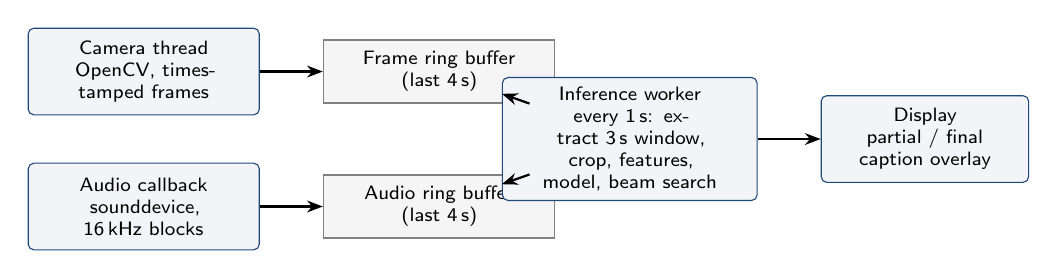
\begin{tikzpicture}[
  node distance=6mm and 8mm,
  th/.style={draw=lsblue, rounded corners=2pt, fill=lsblue!6, align=center,
             font=\scriptsize\sffamily, minimum height=11mm, text width=27mm},
  buf/.style={draw=black!50, fill=black!4, align=center, font=\scriptsize\sffamily,
              minimum height=8mm, text width=27mm},
  ar/.style={-{Stealth[length=2mm]}, thick}]
\node[th] (cam) {Camera thread\\OpenCV, timestamped frames};
\node[th, below=of cam] (mic) {Audio callback\\sounddevice, 16\,kHz blocks};
\node[buf, right=of cam] (vb) {Frame ring buffer\\(last 4\,s)};
\node[buf, right=of mic] (ab) {Audio ring buffer\\(last 4\,s)};
\node[th, right=of $(vb)!0.5!(ab)$, text width=30mm] (inf) {Inference worker\\every 1\,s: extract 3\,s window,\\crop, features, model, beam search};
\node[th, right=of inf, text width=24mm] (ui) {Display\\partial / final caption overlay};
\draw[ar] (cam) -- (vb); \draw[ar] (mic) -- (ab);
\draw[ar] (vb) -- (inf); \draw[ar] (ab) -- (inf); \draw[ar] (inf) -- (ui);
\end{tikzpicture}
\caption{Threads and buffers of the windowed live-captioning mode.}
\label{fig:live}
\end{figure}

\paragraph{Input and buffering.} A camera thread reads frames with OpenCV and
stores each with a timestamp from a single monotonic clock. A
\texttt{sounddevice} callback appends 16\,kHz audio blocks, also timestamped, to a
ring buffer. Both buffers hold the most recent four seconds, which bounds memory
use (four seconds of $640\times480$ colour frames at 30\,fps is about 110\,MB; the
buffer can store downscaled frames or pre-computed crops to reduce this).

\paragraph{Temporal synchronisation.} Webcams rarely deliver exactly 25\,fps and
may drop frames. For a window covering times $[t_0, t_0+3\,\text{s})$ the worker
selects, for each of the 75 target instants $t_0 + 40k$\,ms, the buffered frame
with the nearest timestamp, and cuts the matching 48{,}000 audio samples. Any
constant offset between the camera and microphone pipelines is measured once
with a hand-clap test (comparing the frame where the hands meet with the audio
onset) and subtracted \rec.

\paragraph{Windowing and preprocessing.} Every second the worker processes the
latest 3\,s window, matching the duration of GRID training utterances and giving
$T=75$, which satisfies the CTC length condition (\cref{eq:ctc-cond}). Face Mesh
runs on each new frame as it arrives rather than once per window, so each frame is
processed only once even though windows overlap; the crop smoothing uses an
exponential moving average over past frames. Audio features are computed with
the stored training statistics.

\paragraph{Inference and decoding.} The model runs in evaluation mode, with
gradient tracking disabled by \texttt{torch.inference\_mode()}, and its output
is decoded by beam search. If more than half of
the window's frames lack a face, the visual stream is replaced by
$\mathbf{e}_{\text{miss}}$ and the caption is marked ``audio only''.

\paragraph{Partial and final captions.} A simple energy-based voice-activity
detector tracks speech on the audio buffer. While speech continues, the caption
for the latest window is shown as a grey \emph{partial} caption and replaced each
second. When the detector reports at least 500\,ms of silence, the worker decodes
one window aligned to the detected utterance and displays it as a \emph{final}
caption in black, appended to a short caption history. Restricting final
captions to detected utterances avoids the difficult problem of merging text
from overlapping windows.

\paragraph{Errors and missing input.} If the camera or microphone cannot be
opened, the application reports it and continues in the remaining modality
where possible. Exceptions in the inference worker are logged and the window is
skipped, so a single failure does not stop the display loop.

\subsection{Latency, cost and memory}
Caption latency in Mode~B is the sum of waiting for the window to fill (up to
1\,s for partial captions, the end-of-speech delay for final ones), Face Mesh on
the latest frames, and model and beam-search time. The 3D convolutions over 75
frames dominate model cost; the per-window cost is the same as one test
utterance and will be measured as described in \cref{sec:evaluation}. Real-time
audio-visual recognition on modest hardware is still an active research
problem~\cite{ryumin2023,aripin2024}, so these measurements, rather than
assumptions, will decide the final window settings. If latency
is too high, the team will, in order: run inference every 1.5\,s instead of 1\,s,
reduce beam width, run the model on a GPU, or quantise the model weights.

\subsection{Testing the application}
\begin{itemize}
  \item \textbf{Pre-recorded clips.} Held-out GRID test clips are played through
        Mode~A and through Mode~B (by feeding the file to the buffers in real time).
        Their captions must match those produced by the evaluation script for the
        same clips, which confirms that the application path is equivalent to the
        evaluated path.
  \item \textbf{Live input.} Team members read GRID-grammar sentences to the
        webcam in a quiet room and with played-back background noise. Because the
        model is trained on GRID, it is expected to work only on GRID-like sentences
        spoken in similar framing; free conversation is outside its training
        distribution, and the demonstration will say so.
  \item \textbf{Failure cases.} Covering the mouth, turning the head and leaving the
        frame must produce ``audio only'' captions rather than crashes.
\end{itemize}

% =====================================================================
\section{Additional Objectives: Emotion Detection and Language Identification}
\label{sec:extensions}
% =====================================================================

The proposal includes emotion detection (objective~3) and spoken-language
identification (objective~4) \spec. Neither can be trained on GRID alone:
GRID has no emotion labels, and all of its sentences are in English with one
fixed grammar~\cite{cooke2006}. Both are therefore planned as \emph{separate,
optional modules} with their own data, models and evaluation. They share
preprocessing code with the core system but do not change the speech-recognition
architecture or its results, and work on them begins only after the core
milestones in \cref{sec:schedule} are met.

\subsection{Emotion detection from facial movement}
\paragraph{Approach.} The literature reviewed in the proposal selects Face Mesh
landmarks that correspond to Facial Action Coding System regions and converts
them into compact geometric feature vectors, with reported classification
accuracies of up to 97\% on their data~\cite{siam2022}. LipScribe would follow
the same route \tbd:
\begin{enumerate}
  \item reuse the Face Mesh landmarks already computed by the visual pipeline;
  \item compute geometric features per frame---normalised distances (mouth
        width and opening, eyebrow-to-eye distance, eye aperture) and angles
        between landmark triples---after aligning faces to remove head pose and
        scale;
  \item summarise their temporal changes over an utterance with statistics
        (mean, range, velocity) or a small LSTM;
  \item classify with a lightweight model (for example a random forest or
        multilayer perceptron from scikit-learn) into a small set of emotion
        categories.
\end{enumerate}

\paragraph{Data required.} An emotion-labelled audio-visual dataset is
required. Candidates include CREMA-D~\cite{cao2014} and RAVDESS~\cite{livingstone2018},
both of which provide acted emotional speech with frontal video; the team would
confirm licence terms before use. Evaluation would again use speaker-disjoint
splits and report per-class accuracy and a confusion matrix.

\paragraph{Limitations.} Facial movement while speaking is dominated by
articulation, so mouth landmarks partly reflect \emph{what} is said rather than
how the speaker feels. Acted emotions in such datasets are more exaggerated than
natural ones, facial expression is not a reliable indicator of internal emotional
state, and expressions vary across individuals and cultures. Any emotion output
would be presented as an experimental label, not as a statement about the user.

\paragraph{Integration, if completed.} A separate classification head operating
on landmark features, displayed as a tag next to each final caption. It would not
share loss or weights with the speech recogniser.

\subsection{Spoken-language identification}
\paragraph{Approach.} Language identification predicts which language an
utterance is spoken in. A natural design would add a separate utterance-level
classification head to the existing encoders: time-pool the fused representation
$\mathbf{F}$ and apply a linear classifier over the candidate languages, trained
with cross-entropy alongside or after CTC training \tbd. Audio carries most of the
evidence; the proposal's interest is whether lip movements add to it, since visual
speech patterns differ between languages~\cite{aripin2024,kanavnet2026}.

\paragraph{Data required.} Multilingual audio-visual data with language labels is
essential, and recognising speech (not just identifying the language) in each
additional language would need transcribed data and an extended character
vocabulary. Candidate sources are the multilingual MuAViC corpus~\cite{anwar2023}
or language-specific corpora such as those used for Indonesian and Kannada
lipreading~\cite{aripin2024,kanavnet2026}, subject to availability and licensing.
A locally recorded set of short phrases in English and a Ugandan language could
serve as a small qualitative test, with participants' informed consent.

\paragraph{Limitations.} A model trained on GRID has seen one language, a 51-word
vocabulary and studio conditions. It cannot be expected to transfer to other
languages, accents or scripts without new training data. Language identification
on short utterances is also confounded by speaker identity if each language is
spoken by different people, so speaker-disjoint evaluation is again required.

\subsection{Summary of scope}
\begin{table}[H]
\centering
\caption{Core deliverable versus optional extensions.}
\label{tab:scope}
\small
\begin{tabularx}{\textwidth}{@{}p{3.2cm}XXp{2.2cm}@{}}
\toprule
\textbf{Capability} & \textbf{Data} & \textbf{Model change} & \textbf{Status} \\
\midrule
Audio-visual speech recognition & GRID + MUSAN & Full model (\cref{sec:model}) & Core \\
Emotion detection & Emotion-labelled AV corpus (e.g.\ CREMA-D, RAVDESS) & Separate landmark-feature classifier & Optional \\
Language identification & Multilingual AV corpus with language labels & New utterance-level head; new vocabulary for multilingual ASR & Optional \\
\bottomrule
\end{tabularx}
\end{table}

% =====================================================================
\section{Implementation Schedule and Milestones}
\label{sec:schedule}
% =====================================================================

The schedule covers the six-week capstone period and is ordered by dependency:
no model can be trained before the data are verified, and no fusion experiment is
meaningful before both single-modality baselines work. Training runs are long,
so they are started as early as possible and overlap with development of the
next component. The optional extensions are scheduled only in slack time after
the core system is complete. \Cref{fig:gantt} shows the timeline and
\cref{tab:milestones} the deliverables and completion criteria of each
milestone.

\begin{figure}[H]
\centering
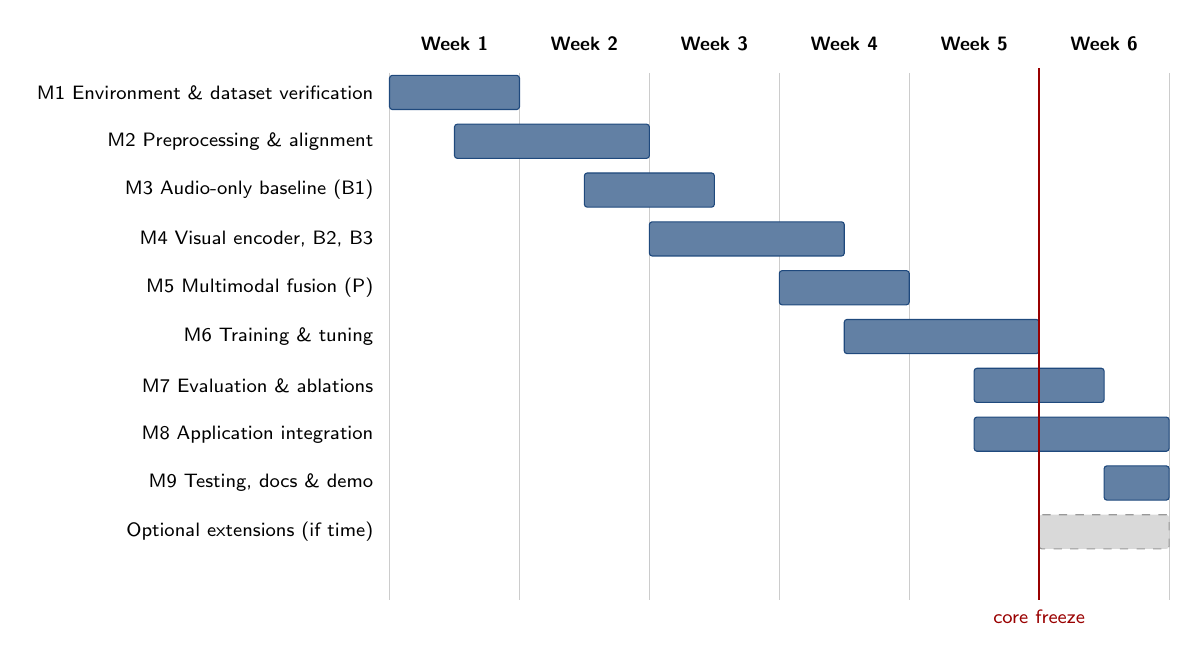
\begin{tikzpicture}[x=1.65cm, y=0.62cm,
  bar/.style={fill=lsblue!70, draw=lsblue, rounded corners=1pt},
  opt/.style={fill=black!15, draw=black!40, rounded corners=1pt, dashed},
  lab/.style={font=\scriptsize\sffamily, anchor=east}]
% grid
\foreach \w in {0,...,6} \draw[black!20] (\w,0.4) -- (\w,-10.4);
\foreach \w in {1,...,6} \node[font=\scriptsize\sffamily\bfseries] at (\w-0.5,1) {Week \w};
% bars: \y, start, end, label
\foreach \y/\s/\e/\l in {
  0/0/1/{M1 Environment \& dataset verification},
  1/0.5/2/{M2 Preprocessing \& alignment},
  2/1.5/2.5/{M3 Audio-only baseline (B1)},
  3/2/3.5/{M4 Visual encoder, B2, B3},
  4/3/4/{M5 Multimodal fusion (P)},
  5/3.5/5/{M6 Training \& tuning},
  6/4.5/5.5/{M7 Evaluation \& ablations},
  7/4.5/6/{M8 Application integration},
  8/5.5/6/{M9 Testing, docs \& demo}} {
  \draw[bar] (\s,-\y-0.35) rectangle (\e,-\y+0.35);
  \node[lab] at (-0.05,-\y) {\l};
}
\draw[opt] (5,-9-0.35) rectangle (6,-9+0.35);
\node[lab] at (-0.05,-9) {Optional extensions (if time)};
\draw[red!60!black, thick] (5,0.5) -- (5,-10.4) node[below, font=\scriptsize\sffamily, text=red!60!black] {core freeze};
\end{tikzpicture}
\caption{Gantt-style implementation timeline. Dashed bar: optional work, started only
after the core system is frozen at the end of week~5.}
\label{fig:gantt}
\end{figure}

{\small
\setlength{\tabcolsep}{4pt}
\begin{longtable}{@{}p{0.8cm}p{3.0cm}p{1.1cm}p{4.4cm}p{5.1cm}@{}}
\caption{Milestones, dependencies, deliverables and completion criteria.}\label{tab:milestones}\\
\toprule
\textbf{ID} & \textbf{Milestone} & \textbf{Needs} & \textbf{Deliverables} & \textbf{Completion criteria} \\
\midrule
\endfirsthead
\multicolumn{5}{@{}l}{\small\itshape \Cref{tab:milestones} continued}\\
\toprule
\textbf{ID} & \textbf{Milestone} & \textbf{Needs} & \textbf{Deliverables} & \textbf{Completion criteria} \\
\midrule
\endhead
\bottomrule
\endfoot
M1 & Environment setup and dataset verification & -- &
Repository skeleton, pinned environment, raw GRID and MUSAN, integrity report, \texttt{splits.csv} &
Every member runs the test suite; integrity report lists usable utterances per speaker; speaker sets disjoint; GPU access confirmed \\
M2 & Preprocessing and data alignment & M1 &
Cached mouth crops, 16\,kHz audio, manifest, noise mixer, fixed noisy test sets, normalisation statistics, data loader &
Crop contact sheets reviewed; noise-mixing tests pass; one batch loads with consistent lengths; train/infer parity test passes \\
M3 & Baseline implementation (audio-only) & M2 &
Training and evaluation scripts, B1 checkpoint &
B1 overfits 8 utterances; full B1 run completes and is evaluated at all five SNRs \\
M4 & Visual and audio encoder development & M2 &
Visual encoder V1, B2 and B3 checkpoints &
Encoder shape tests pass; B2 validation CER falls clearly below that of an untrained model; B3 evaluated at all SNRs \\
M5 & Multimodal fusion & M3, M4 &
Attention fusion, gate, modality dropout, first P checkpoint &
Fusion unit tests pass; no NaN under full-modality dropout; P trains stably \\
M6 & Training and hyperparameter tuning & M5 &
Tuned P configuration; final checkpoints of B1--B3 and P &
Learning-rate and modality-dropout sweeps logged; best configuration chosen on validation data only \\
M7 & Evaluation and ablation studies & M6 &
Per-SNR WER/CER tables and plots, ablations X1--X3, gate analysis, latency measurements &
All core models evaluated on identical test audio; every number traceable to a config and checkpoint \\
M8 & Application integration & M3 (Mode A), M6 (final) &
Gradio Mode A, live Mode B, \texttt{transcribe.py} &
Mode A captions match the evaluation script on test clips; Mode B runs for 5 minutes without error \\
M9 & Testing, documentation and demonstration & M7, M8 &
Final report, README, demonstration rehearsal, frozen release tag &
Fresh clone installs and reproduces one evaluation; demonstration rehearsed with a recorded fallback clip \\
\end{longtable}
}

\paragraph{Prioritisation.} If the schedule slips, work is dropped in this order:
optional extensions; experiments X4--X6; Mode B live captioning (Mode A remains);
multiple seeds. Baselines B1--B3, the proposed model P, the per-SNR evaluation and
ablations X1--X3 are never dropped, because they constitute the core contribution
described in the proposal.

\paragraph{Team organisation.} Work is divided into three pairs \rec: a data pair
(M1--M2, noise and integrity), a model pair (encoders, fusion, training) and an
application pair (inference script, Gradio interface, live mode, tests), with all
members contributing to evaluation and the report. A short weekly review checks
completion criteria and re-plans.

% =====================================================================
\section{Risks, Limitations and Mitigation}
\label{sec:risks}
% =====================================================================

\Cref{tab:risks} lists the main implementation risks, an assessment of their
likelihood and impact, and the planned mitigation. Assessments are the team's
judgement at the planning stage and will be reviewed weekly.

{\small
\setlength{\tabcolsep}{4pt}
\renewcommand{\arraystretch}{1.15}
\begin{longtable}{@{}p{3.5cm}p{1.4cm}p{10.2cm}@{}}
\caption{Implementation risks and mitigation strategies (L/I = likelihood/impact, rated H = high, M = medium, L = low).}\label{tab:risks}\\
\toprule
\textbf{Risk} & \textbf{L / I} & \textbf{Mitigation} \\
\midrule
\endfirsthead
\multicolumn{3}{@{}l}{\small\itshape \Cref{tab:risks} continued}\\
\toprule
\textbf{Risk} & \textbf{L / I} & \textbf{Mitigation} \\
\midrule
\endhead
\bottomrule
\endfoot
Limited compute resources & H / H &
Confirm GPU access in week~1; use mixed precision and cached crops; develop on a
subset of speakers; keep the model moderate in size; drop optional experiments
first (\cref{sec:schedule}). \\
Long training times & H / M &
Start B1 in week~2 and overlap training with development; use early stopping;
schedule long runs overnight; checkpoint every epoch so runs can be resumed. \\
Misaligned audio and video & M / H &
Never drop frames during cropping; integrity check of durations; automated
train/infer parity test; time-shift sanity test (\cref{tab:tests}); clap-test
calibration for live input. \\
CTC training instability & M / H &
Learning-rate warm-up, gradient clipping and \texttt{zero\_infinity}; assert the
length condition (\cref{eq:ctc-cond}); overfit a tiny batch before full runs;
log non-finite losses. \\
Token distribution issues & M / L &
The blank symbol dominates CTC outputs and GRID's grammar makes some characters
much more frequent; monitor CER per word slot and the share of blank predictions;
inspect the letter slot separately, as it is the hardest. \\
Speaker leakage & L / H &
Speaker-level split stored in one file; loader refuses overlapping speakers;
disjointness unit test; statistics from training speakers only. \\
Poor generalisation to unseen speakers & M / H &
Crop jitter, horizontal flip, dropout and weight decay; model selection on
held-out validation speakers; report per-speaker results honestly. \\
Mouth detection failure (lighting, head pose, occlusion) & M / M &
GRID is frontal and well lit, so this mainly affects the live demo; interpolate
short gaps; fall back to audio-only captions using $\mathbf{e}_{\text{miss}}$; good
lighting and frontal camera position for the demonstration. \\
Attention fusion fails to improve performance & M / H &
Report the outcome truthfully; diagnose with gate analysis, test-time modality
ablations and the checklist in \cref{sec:evaluation}; tune modality dropout;
B3 remains a working fused system. \\
Excessive inference latency & M / M &
Measure early on the demo machine; increase window hop, reduce beam width, use a
GPU or quantise; Mode A batch captioning as the guaranteed fallback. \\
Limited multilingual generalisation & H / L (core) &
Treat language identification as an optional extension with its own data; state
clearly that the core model covers GRID English only. \\
Domain gap between GRID and live speech & H / M &
Restrict the demonstration to GRID-grammar sentences; explain the closed
vocabulary; identify larger datasets (e.g.\ those in~\cite{afouras2022}) as future
work. \\
Privacy of camera and microphone input & M / H &
Process all input locally; do not store live video or audio by default; show a
clear on-screen indicator while capturing; record any demonstration data only
with written consent and delete it after the project; never upload live input to
third-party services. \\
\end{longtable}
}

\subsection{Limitations of the planned system}
Even if every risk is managed, the system will have known limitations. GRID's
fixed grammar and 51-word vocabulary~\cite{cooke2006} make the recognition task far
easier than open captioning, so a low WER on GRID does not imply comparable
accuracy on lectures or meetings~\cite{afouras2022}. Synthetic additive noise does
not reproduce reverberation, competing speakers or microphone distortion. The
visual front-end assumes a roughly frontal, unoccluded face, which the literature
identifies as an open problem~\cite{ameer2025,kanavnet2026}. The final report will
state these limitations alongside the results.

% =====================================================================
\section{Expected Deliverables}
\label{sec:deliverables}
% =====================================================================

The proposal commits to a clean inference script and a simple web
demonstration \spec. \Cref{tab:deliverables} lists the full set of software
artefacts the implementation will produce and the evidence that will show each
one works.

{\small
\setlength{\tabcolsep}{4pt}
\begin{longtable}{@{}p{3.5cm}p{5.4cm}p{6.2cm}@{}}
\caption{Software deliverables and evidence of completion.}\label{tab:deliverables}\\
\toprule
\textbf{Deliverable} & \textbf{Content} & \textbf{Evidence that it works} \\
\midrule
\endfirsthead
\multicolumn{3}{@{}l}{\small\itshape \Cref{tab:deliverables} continued}\\
\toprule
\textbf{Deliverable} & \textbf{Content} & \textbf{Evidence that it works} \\
\midrule
\endhead
\bottomrule
\endfoot
Modular source code & Python package \texttt{lipscribe/} with \texttt{data}, \texttt{preprocessing}, \texttt{models}, \texttt{decoding}, \texttt{evaluation} and \texttt{app} sub-packages &
Package installs with \texttt{pip install -e .}; modules imported by scripts and tests \\
Data-preparation scripts & \texttt{verify\_dataset.py}, \texttt{extract\_mouths.py}, \texttt{prepare\_audio.py}, \texttt{make\_noisy\_test.py}, \texttt{compute\_stats.py} &
Integrity report, manifest and contact sheets generated from raw data by one documented command sequence \\
Configuration files & One YAML file per experiment in \texttt{configs/} &
Every reported run has a committed configuration \\
Training and evaluation scripts & \texttt{train.py}, \texttt{evaluate.py}, \texttt{transcribe.py} &
Re-running \texttt{evaluate.py} on a released checkpoint reproduces its reported WER \\
Model checkpoints & Best checkpoints of B1, B2, B3 and P (and ablations) &
Load without error and match logged validation scores \\
Baseline implementations & Audio-only, visual-only and concatenation models &
Evaluated at all five SNRs with the same protocol as P \\
Experiment logs and outputs & TensorBoard logs, \texttt{results.csv}, per-SNR tables, WER-vs-SNR and gate plots &
Each table entry traceable to a run directory \\
Automated tests & \texttt{pytest} suite (\cref{tab:tests}) &
All tests pass on a fresh environment; test report included \\
Captioning demonstration & Gradio Mode A and live Mode B &
Live demonstration plus a recorded fallback video; Mode A matches \texttt{evaluate.py} on test clips \\
Setup and execution instructions & \texttt{README.md}, \texttt{requirements.txt}, data download guide &
A team member not involved in setup reproduces one evaluation from a fresh clone \\
Final technical report & Methods, results, ablations, limitations &
Submitted; all results come from logged runs \\
\end{longtable}
}

% =====================================================================
\section{Conclusion}
\label{sec:conclusion}
% =====================================================================

This document has translated the LipScribe proposal into an implementation plan.
The system is built from separable modules: a visual stream that uses MediaPipe
Face Mesh to extract stabilised $96\times96$ mouth crops and encodes them with a 3D
convolutional front-end and a BiLSTM; an audio stream that converts 16\,kHz audio
into log-Mel features and encodes them with strided convolutions and a BiLSTM at
the same 25\,fps rate; a cross-modal attention and gating module that combines
the two; and a CTC output layer decoded by prefix beam search. Modality dropout
and multi-condition training with MUSAN noise are the mechanisms through which the
fusion is expected to learn to rely on the lips when the audio degrades.

The architecture, the development stages and the evaluation plan are tied
together by design. Each milestone produces a component with its own tests; the
baselines reuse the same components, so that every comparison isolates one
change; and the per-SNR evaluation on held-out speakers measures exactly the
property the project claims to improve. The same preprocessing code serves
training and the captioning demonstration, so the demonstrated behaviour reflects
the evaluated model.

The plan also states what remains uncertain. The clean-condition target of WER
below 10\% and the expected advantage at 0 and $-5$\,dB are hypotheses to be
tested, not results. Emotion detection and language identification require data
that GRID does not provide and are kept as optional extensions. By completing the
core recogniser first, reporting outcomes faithfully---including any in which
fusion does not help---and documenting every experiment, the team aims to deliver
a working, verifiable audio-visual captioning system within the six-week course.


\clearpage
% ---------------------------------------------------------------- references
% References [1]-[8] reproduce the bibliography of the LipScribe proposal.
% References [9]-[18] were added for this implementation document; they cover
% the datasets, methods and tools that the proposal names but does not cite.
\section*{References}
\addcontentsline{toc}{section}{References}

\subsection*{References from the project proposal}
\begingroup
\renewcommand{\section}[2]{}%
\small
\begin{thebibliography}{99}
\setlength{\itemsep}{3pt}

\bibitem{lipsyncnet2024}
S.~A.~A. Jeevakumari and K.~Dey, ``LipSyncNet: A novel deep learning approach for
visual speech recognition in audio-challenged situations,'' \emph{IEEE Access},
vol.~12, pp.~110891--110904, 2024. DOI: 10.1109/ACCESS.2024.3436931

\bibitem{li2023}
D.~Li, Y.~Gao, C.~Zhu, Q.~Wang, and R.~Wang, ``Improving speech recognition
performance in noisy environments by enhancing lip reading accuracy,''
\emph{Sensors}, vol.~23, no.~4, p.~2053, 2023. DOI: 10.3390/s23042053

\bibitem{aripin2024}
Aripin and A.~Setiawan, ``Indonesian lip-reading detection and recognition based
on lip shape using face mesh and long-term recurrent convolutional network,''
\emph{Applied Computational Intelligence and Soft Computing}, vol.~2024,
p.~6479124, 2024. DOI: 10.1155/2024/6479124

\bibitem{kanavnet2026}
Divya and D.~Suresha, ``KanAVNet: A CNN-BiLSTM-CTC-based audio-visual speech
recognition system for Kannada to assist the hearing impaired,'' \emph{I.J. Image,
Graphics and Signal Processing}, vol.~2, pp.~87--106, 2026.
DOI: 10.5815/ijigsp.2026.02.06

\bibitem{ameer2025}
A.~W.~A. Ameer, P.~Salehpour, and M.~Asadpour, ``Deep transfer learning for lip
reading based on NASNetMobile pretrained model in wild dataset,'' \emph{IEEE
Access}, vol.~13, pp.~11625--11640, 2025. DOI: 10.1109/ACCESS.2024.3470521

\bibitem{afouras2022}
T.~Afouras, J.~S. Chung, A.~Senior, O.~Vinyals, and A.~Zisserman, ``Deep
audio-visual speech recognition,'' \emph{IEEE Transactions on Pattern Analysis and
Machine Intelligence}, vol.~44, no.~12, pp.~8717--8727, 2022.
DOI: 10.1109/TPAMI.2018.2889052

\bibitem{siam2022}
A.~I. Siam, N.~F. Soliman, A.~D. Algarni, F.~E. Abd El-Samie, and A.~Sedik,
``Deploying machine learning techniques for human emotion detection,''
\emph{Computational Intelligence and Neuroscience}, vol.~2022, p.~8032673, 2022.
DOI: 10.1155/2022/8032673

\bibitem{ryumin2023}
D.~Ryumin, D.~Ivanko, and E.~Ryumina, ``Audio-visual speech and gesture recognition
by sensors of mobile devices,'' \emph{Sensors}, vol.~23, no.~4, p.~2284, 2023.
DOI: 10.3390/s23042284

\end{thebibliography}
\endgroup

\subsection*{Additional references introduced in this document}
\begingroup
\renewcommand{\section}[2]{}%
\small
\begin{thebibliography}{99}
\setlength{\itemsep}{3pt}
\makeatletter\setcounter{\@listctr}{8}\makeatother

\bibitem{cooke2006}
M.~Cooke, J.~Barker, S.~Cunningham, and X.~Shao, ``An audio-visual corpus for speech
perception and automatic speech recognition,'' \emph{The Journal of the Acoustical
Society of America}, vol.~120, no.~5, pp.~2421--2424, 2006. DOI: 10.1121/1.2229005

\bibitem{snyder2015}
D.~Snyder, G.~Chen, and D.~Povey, ``MUSAN: A music, speech, and noise corpus,''
arXiv preprint arXiv:1510.08484, 2015.

\bibitem{graves2006}
A.~Graves, S.~Fern\'andez, F.~Gomez, and J.~Schmidhuber, ``Connectionist temporal
classification: Labelling unsegmented sequence data with recurrent neural
networks,'' in \emph{Proc. 23rd International Conference on Machine Learning
(ICML)}, 2006, pp.~369--376. DOI: 10.1145/1143844.1143891

\bibitem{assael2016}
Y.~M. Assael, B.~Shillingford, S.~Whiteson, and N.~de~Freitas, ``LipNet: End-to-end
sentence-level lipreading,'' arXiv preprint arXiv:1611.01599, 2016.

\bibitem{tan2019}
M.~Tan and Q.~V. Le, ``EfficientNet: Rethinking model scaling for convolutional
neural networks,'' in \emph{Proc. 36th International Conference on Machine Learning
(ICML)}, PMLR vol.~97, 2019, pp.~6105--6114.

\bibitem{lugaresi2019}
C.~Lugaresi \emph{et al.}, ``MediaPipe: A framework for building perception
pipelines,'' arXiv preprint arXiv:1906.08172, 2019.

\bibitem{kartynnik2019}
Y.~Kartynnik, A.~Ablavatski, I.~Grishchenko, and M.~Grundmann, ``Real-time facial
surface geometry from monocular video on mobile GPUs,'' arXiv preprint
arXiv:1907.06724, 2019.

\bibitem{cao2014}
H.~Cao, D.~G. Cooper, M.~K. Keutmann, R.~C. Gur, A.~Nenkova, and R.~Verma,
``CREMA-D: Crowd-sourced emotional multimodal actors dataset,'' \emph{IEEE
Transactions on Affective Computing}, vol.~5, no.~4, pp.~377--390, 2014.

\bibitem{livingstone2018}
S.~R. Livingstone and F.~A. Russo, ``The Ryerson Audio-Visual Database of Emotional
Speech and Song (RAVDESS): A dynamic, multimodal set of facial and vocal
expressions in North American English,'' \emph{PLoS ONE}, vol.~13, no.~5,
e0196391, 2018. DOI: 10.1371/journal.pone.0196391

\bibitem{anwar2023}
M.~Anwar, B.~Shi, V.~Goswami, W.-N. Hsu, J.~Pino, and C.~Wang, ``MuAViC: A
multilingual audio-visual corpus for robust speech recognition and robust
speech-to-text translation,'' in \emph{Proc. Interspeech}, 2023.
arXiv:2303.00628

\end{thebibliography}
\endgroup


\end{document}
